\documentclass[11pt]{article}
\usepackage{physoly}
\usepackage[utf8]{vietnam} % For Vietnamese translation
\usepackage{multicol}
\usepackage{wasysym}
\usepackage{titling}
\usepackage{epstopdf}
\usepackage{physics}
\usepackage{enumitem}
\usepackage{lipsum}
% \usepackage[T1]{fontenc}
\usepackage{siunitx}
\usepackage{dcolumn, amsmath, amssymb}
\usepackage[section]{placeins}
\usepackage{hyperref}
\setlength{\parskip}{\baselineskip}%
\usepackage[inline]{asymptote}
\usepackage{multirow}
\setlength{\parindent}{0pt}
\renewcommand{\quote}{\list{}{\rightmargin=\leftmargin\topsep=0pt}\item\relax}
\usepackage{changepage}   % for the adjustwidth environment
\usetikzlibrary{positioning,fadings,through}

\definecolor{left} {HTML}{001528}

\usepackage{hyperref}
\hypersetup{
    colorlinks=true,
    linkcolor=blue,
    filecolor=magenta,      
    urlcolor=blue,
}
\usepackage{tikz}
\tikzset{%
  3d/.unknown/.code={%
    \ifx\cx\relax%
      \let\cx=\pgfkeyscurrentname%
    \else%
       \ifx\cy\relax%
         \let\cy=\pgfkeyscurrentname%
       \else%
         \let\cz=\pgfkeyscurrentname%
       \fi%
     \fi% 
    }
}
\tikzdeclarecoordinatesystem{3d}{%
  \let\cx=\relax\let\cy=\relax\let\cz=\relax%
  \tikzset{3d/.cd,#1}%
  % Not a proper perspective calculation
  \pgfmathparse{1.05^(\cx)*1.05^(\cz)}\let\cf=\pgfmathresult%
  \pgfpointxyz{(\cx)*\cf}{(\cy)*\cf}{(\cz)*\cf}%
}
\usetikzlibrary{shapes.geometric, arrows}
\tikzstyle{arrow} = [thick,->,>=stealth]
\usetikzlibrary{decorations.pathmorphing,patterns}
\tikzstyle{spring}=[thick,decorate,decoration={zigzag,pre length=0.1cm,post
  length=0.1cm,segment length=6}]
\usepackage{subfigure}

\usepackage{tikz}
\def\width{19}
\def\hauteur{15}
\usetikzlibrary{shapes,positioning,intersections,quotes}
\usepackage{fancyhdr}

\pagestyle{fancy}
\fancyhf{}
\rhead{Online Physics Olympiad 2024 - Đáp án vòng Open}
\lhead{Ngày 12 - 14, tháng 8, năm 2024}
\rfoot{Trang \thepage}
\title{Đề OPhO}

\begin{document}

\begin{titlepage}
    \begin{center}
        
        \Huge
        \textbf{2024 Online Physics Olympiad: \\
        Đáp án vòng Open}
        
        \vspace{0.5cm}
        
        \begin{center}
            
\includegraphics[width=0.6\linewidth]{OPhO Logo, White BKGD.png}
        \end{center}
        \end{center}


\section*{Nhà tài trợ}

\vspace{-0.5cm}

Cuộc thi này sẽ không thể thành công nếu thiếu đi sự trợ giúp từ các nhà tài trợ, những người đã đóng góp rất nhiều cho vật lý, toán và giáo dục.
% This competition could not be possible without the help of our sponsors, who are all doing great things in physics, math, and education.
\begin{center}
    
\includegraphics[width = 4cm]{sponsors/jane-street.png}\qquad
\includegraphics[width = 5cm]{sponsors/wolfram.png}\qquad
\includegraphics[width = 5cm]{sponsors/awesome-math.png}\\ 
    
    
\includegraphics[width=2cm]{sponsors/btbb.png}\qquad
\includegraphics[width=2.5cm]{sponsors/physolymp.jpg}\qquad
\includegraphics[width=4cm]{sponsors/aops.png}
\end{center}
\end{titlepage}
\newpage
\section*{Hướng dẫn}
Nếu bạn muốn yêu cầu làm rõ, vui lòng sử dụng \href{https://forms.gle/adb6hNCrQFhHVvVe6}{biểu mẫu này}. Để xem tất cả các giải thích, xem \href{https://docs.google.com/document/d/1W71dFM-XDmuTxXJ_MJ3QfSdE_xxISvIw58FZh1wYEIk/edit}{tài liệu này}.
\begin{itemize}
    \item Sử dụng $g=9.8\;\mathrm{m/s^2}$ trong cuộc thi này, \textbf{trừ khi có quy định khác}. Xem bảng hằng số ở trang tiếp theo để biết các hằng số khác.
    \item Bài kiểm tra này có 35 câu hỏi ngắn. Mỗi bài toán sẽ có ba lần thử.
    \item Trọng số của mỗi câu hỏi phụ thuộc vào hệ thống chấm điểm của chúng tôi được tìm thấy \href{https://opho.physoly.tech/static/files/rules24.pdf}{ở đây}. Nói đơn giản, các câu hỏi sau có giá trị cao hơn, và tổng số điểm từ một câu hỏi nhất định sẽ giảm theo số lần bạn thử giải bài toán cũng như số đội giải được nó.
    \item Bất kỳ thành viên nào trong đội đều có thể nộp bài. Việc chia nhỏ công việc hay làm mỗi bài toán cùng nhau là tùy thuộc vào bạn. Lưu ý rằng sau khi bạn đã nộp bài, các đồng đội của bạn phải làm mới trang của họ trước khi họ có thể thấy nó.
    \item Câu trả lời nên chứa \textbf{ba} chữ số có nghĩa, trừ khi có quy định khác. Tất cả các câu trả lời trong phạm vi \(1\%\) sẽ được chấp nhận.
    \item Khi nộp câu trả lời bằng ký hiệu khoa học, vui lòng sử dụng dạng số mũ. Nói cách khác, nếu câu trả lời của bạn cho một bài toán là $A\times 10^B$, vui lòng nhập $A\text{e}B$ vào cổng nộp bài.
    \item Một máy tính cầm tay khoa học hoặc đồ thị tiêu chuẩn \textit{có thể} được sử dụng. Các hệ thống đại số máy tính và công nghệ như Wolfram Alpha hoặc TI Nspire sẽ không cần thiết, nhưng có thể được sử dụng.
    \item Bạn \textit{được phép} sử dụng Wikipedia hoặc sách trong kỳ thi này. Hỏi xin trợ giúp trên các diễn đàn trực tuyến hoặc từ giáo viên của bạn sẽ bị coi là gian lận và có thể dẫn đến việc cấm tham gia các cuộc thi trong tương lai.
    \item Những người đạt điểm cao nhất từ cuộc thi này sẽ đủ điều kiện tham gia \textit{Cuộc thi Mời của Olympic Vật lý Trực tuyến}, là một kỳ thi theo phong cách olympic. Thông tin thêm sẽ được cung cấp cho những người đủ điều kiện sau khi kết thúc \textit{Cuộc thi Mở}.
    \item Nói chung, trả lời bằng đơn vị SI (mét, giây, kilogram, watt, v.v.) trừ khi có quy định khác. Vui lòng nhập tất cả các góc bằng độ trừ khi có quy định khác.
    \item Nếu câu hỏi yêu cầu đưa ra câu trả lời dưới dạng phần trăm và câu trả lời của bạn là ``$x$\%”, vui lòng nhập giá trị $x$ vào biểu mẫu nộp bài.
    \item Không đặt đơn vị trong câu trả lời của bạn trên cổng nộp bài! Nếu câu trả lời của bạn là ``$x$ mét”, chỉ nhập giá trị $x$ vào cổng nộp bài.
    \item \textbf{Không truyền đạt thông tin cho bất kỳ ai khác ngoài các thành viên trong đội của bạn trước ngày 25 tháng 8 năm 2024}.
\end{itemize}

\newpage
\section*{Danh mục hằng số}
\begin{multicols}{2}
\begin{itemize}
    \item Khối lượng proton, $m_p = 1.67\cdot 10^{-27}\;\mathrm{kg}$
    \item Khối lượng neutron, $m_n = 1.67 \cdot 10^{-27}\;\mathrm{kg}$
    \item Khối lượng electron, $m_e = 9.11 \cdot 10^{-31}\;\mathrm{kg}$
    \item Hằng số Avogadro, $N_0 = 6.02 \cdot 10^{23}\;\mathrm{mol^{-1}}$
    \item Hằng số khí lý tưởng, $R = 8.31\;\mathrm{J/(mol\cdot K)}$
    \item Hằng số Boltzmann, $k_B = 1.38\cdot 10^{-23}\;\mathrm{J/K}$
    \item Điện tích hạt electron, $e = 1.60 \cdot 10^{-19}\;\mathrm{C}$
    \item 1 electron volt, $1\;\mathrm{eV} = 1.60\cdot 10^{-19}\;\mathrm{J}$
    \item Vận tốc ánh sáng, $c = 3.00 \cdot 10^8\;\mathrm{m/s}$
    \item Hằng số hấp dẫn, \[G = 6.67\cdot 10^{-11}\;\mathrm{(N\cdot m^2)/kg^2}\]
    \item Khối lượng mặt trời
    \[M_{\odot} = 1.988\cdot 10^{30}\;\mathrm{kg}\]
    \item Gia tốc trọng trường, $g = 9.8\;\mathrm{m/s^2}$
    \item 1 đơn vị nguyên tử khối, \[1\;\mathrm{u} = 1.66 \cdot 10^{-27}\;\mathrm{kg} = 931\;\mathrm{MeV/c^2}\]
    \item Hằng số Planck, 
        \[h = 6.63 \cdot 10^{-34}\;\mathrm{J\cdot s} = 4.41\cdot 10^{-15}\;\mathrm{eV\cdot s}\]
    \item Hằng số điện môi của chân không, \[\epsilon_0 = 8.85 \cdot 10^{-12}\;\mathrm{C^2/(N\cdot m^2)}\]
    \item Hằng số lực Coulomb,
    \[k = \frac{1}{4\pi\epsilon_0} = 8.99 \cdot 10^9\;\mathrm{(N\cdot m^2)/C^2}\]
    \item Độ từ thẩm của chân không, \[\mu_0 = 4\pi\cdot 10^{-7}\;\mathrm{T\cdot m/A}\]
    \item Hằng số từ, 
    \[ \frac{\mu_0}{4\pi} = 1\cdot 10^{-7}\;\mathrm{(T\cdot m)/A}\]
    \item Áp suất 1 atmosphere ,
    \[1\;\mathrm{atm} = 1.01 \cdot 10^5\;\mathrm{N/m^2} = 1.01\cdot 10^5\;\mathrm{Pa}\]
    \item Hằng số dịch chuyển Wien, $b = 2.9\cdot 10^{-3}\;\mathrm{m\cdot K}$
    \item Hằng số Stefan-Boltzmann, \[\sigma = 5.67\cdot 10^{-8}\;\mathrm{W/m^2/K^4}\]
\end{itemize}
\end{multicols}
\newpage
\normalsize
\begin{center}
    \Large 
    \textbf{Problems}
\end{center}

\begin{solution}
    The car's initial velocity is $v_0 =X/T$. Using $v^2 = 2 a \Delta x$, we find its acceleration is $a=\frac{X}{2T^2}$. Therefore, the distance the car travels in time $T$ is 

    $$v_0 T - \frac{1}{2} a T^2 = \frac{3}{4} X= 30.0 \ m$$

    You do not get hit by the car, and you are $\boxed{2.0 \ \mathrm{m}}$ away from the car when you finish crossing the street.

\end{solution}
\begin{solution}
    The car's initial velocity is $v_0 =X/T$. Using $v^2 = 2 a \Delta x$, we find its acceleration is $a=\frac{X}{2T^2}$. Therefore, the distance the car travels in time $T$ is 

    $$v_0 T - \frac{1}{2} a T^2 = \frac{3}{4} X= 30.0 \ m$$

    You do not get hit by the car, and you are $\boxed{2.0 \ \mathrm{m}}$ away from the car when you finish crossing the street.

\end{solution}

\begin{solution} Ý tưởng chính là viết ánh sáng phân cực phẳng như sự chồng chất của hai sóng ánh sáng phân cực tròn có cùng tần số.Ý tưởng chính là viết ánh sáng phân cực phẳng như sự chồng chất của hai sóng ánh sáng phân cực tròn có cùng tần số.
\begin{center}
    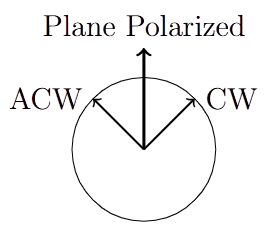
\includegraphics[width=0.25\textwidth]{solutions/figures/polarization-decomposition.png}
\end{center}
    
Sau khi đi qua dung dịch, do chúng có chỉ số khúc xạ khác nhau là $n_L$ và $n_R$, độ chênh lệch pha giữa chúng được cho bởi
$$\frac{\phi}{2\pi} = \frac{L}{\lambda_{\text{medium}}} = \frac{L}{\frac{\lambda}{n}} \implies \Delta \phi = \frac{2\pi}{\lambda}L\Delta n$$
    
Tuy nhiên, cần lưu ý rằng đây là độ dịch pha chứ không phải góc quay.

\begin{center}
    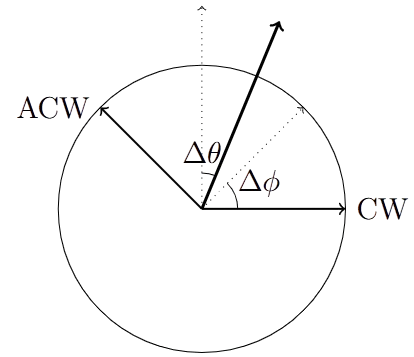
\includegraphics[width=0.3\textwidth]{solutions/figures/rotation-shift.png}
\end{center}
    
Do đó $\Delta \theta = \frac{1}{2}\Delta \phi = \frac{\pi}{\lambda} L \Delta n$. Thay các giá trị vào ta được $\boxed{\Delta \theta = \frac{3\pi}{2} \approx 4.71\;\mathrm{rad}}$.

\end{solution}
\begin{solution} Ý tưởng chính là viết ánh sáng phân cực phẳng như sự chồng chất của hai sóng ánh sáng phân cực tròn có cùng tần số.Ý tưởng chính là viết ánh sáng phân cực phẳng như sự chồng chất của hai sóng ánh sáng phân cực tròn có cùng tần số.
\begin{center}
    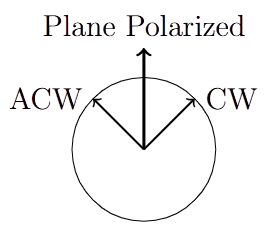
\includegraphics[width=0.25\textwidth]{solutions/figures/polarization-decomposition.png}
\end{center}
    
Sau khi đi qua dung dịch, do chúng có chỉ số khúc xạ khác nhau là $n_L$ và $n_R$, độ chênh lệch pha giữa chúng được cho bởi
$$\frac{\phi}{2\pi} = \frac{L}{\lambda_{\text{medium}}} = \frac{L}{\frac{\lambda}{n}} \implies \Delta \phi = \frac{2\pi}{\lambda}L\Delta n$$
    
Tuy nhiên, cần lưu ý rằng đây là độ dịch pha chứ không phải góc quay.

\begin{center}
    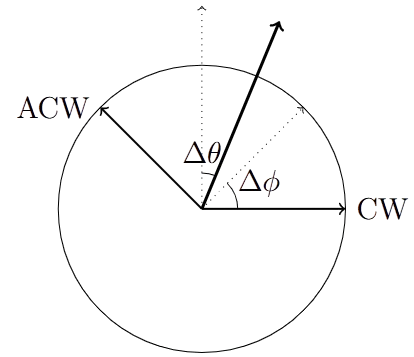
\includegraphics[width=0.3\textwidth]{solutions/figures/rotation-shift.png}
\end{center}
    
Do đó $\Delta \theta = \frac{1}{2}\Delta \phi = \frac{\pi}{\lambda} L \Delta n$. Thay các giá trị vào ta được $\boxed{\Delta \theta = \frac{3\pi}{2} \approx 4.71\;\mathrm{rad}}$.

\end{solution}

\begin{solution}
Thời gian để quả bóng được thả từ bề mặt đến đáy hồ là

$$a = g\bigg(\frac{\rho_b - \rho_p}{\rho_b}\bigg) = rg$$

$$t = \sqrt{\frac{2d}{rg}}$$


Thời gian để quả bóng được thả từ trên không đến bề mặt hồ là

$$t_1 = \sqrt{\frac{2h}{g}}$$

$$v_1 = at_1 = \sqrt{2gh}$$

$$v_2 = \sqrt{v_1^2 + 2ad} = \sqrt{2gh + 2rgd}$$

$$t_2 = \frac{v_2 - v_1}{a} = \frac{\sqrt{2gh + 2rgd} - \sqrt{2gh}}{rg}$$

Điều kiện $t_1 + t_2 = t$ phải được thỏa mãm

$$\sqrt{\frac{2d}{rg}} = \sqrt{\frac{2h}{g}} + \frac{\sqrt{2gh + 2rgd} - \sqrt{2gh}}{rg}\longrightarrow\frac{\sqrt{2rd}}{r\sqrt{g}} = \frac{r\sqrt{2h} + \sqrt{2h + 2rd} - \sqrt{2h}}{r\sqrt{g}}$$

$$\sqrt{2rd} - (r-1)\sqrt{2h} = \sqrt{2h + 2rd}\longrightarrow 2rd - 4(r-1)\sqrt{rdh} + 2h(r-1)^2 = 2h + 2rd$$

$$h(r-1)^2 - 2(r-1)\sqrt{rdh} = h\longrightarrow 2(r-1)\sqrt{rdh} = h(r-1)^2 - h$$

$$\sqrt{d} = \frac{h(r-1)}{2\sqrt{rh}} - \frac{h}{2\sqrt{rh}(r-1)}\longrightarrow d = \frac{h(r-1)^2}{4r} - \frac{h}{2r} + \frac{h}{4r(r-1)^2}$$

$$d = \frac{(r-1)^4-2(r-1)^2 + 1}{4r(r-1)^2} h$$

$$d = \frac{r(r-2)^2}{4(r-1)^2}h = \frac{r^3 - 4r^2 + 4r}{4r^2-8r+4}h$$

Đáp án lúc này là $1-4+4+4-8+4=\boxed{1}$.
\end{solution}
\begin{solution}
Thời gian để quả bóng được thả từ bề mặt đến đáy hồ là

$$a = g\bigg(\frac{\rho_b - \rho_p}{\rho_b}\bigg) = rg$$

$$t = \sqrt{\frac{2d}{rg}}$$


Thời gian để quả bóng được thả từ trên không đến bề mặt hồ là

$$t_1 = \sqrt{\frac{2h}{g}}$$

$$v_1 = at_1 = \sqrt{2gh}$$

$$v_2 = \sqrt{v_1^2 + 2ad} = \sqrt{2gh + 2rgd}$$

$$t_2 = \frac{v_2 - v_1}{a} = \frac{\sqrt{2gh + 2rgd} - \sqrt{2gh}}{rg}$$

Điều kiện $t_1 + t_2 = t$ phải được thỏa mãm

$$\sqrt{\frac{2d}{rg}} = \sqrt{\frac{2h}{g}} + \frac{\sqrt{2gh + 2rgd} - \sqrt{2gh}}{rg}\longrightarrow\frac{\sqrt{2rd}}{r\sqrt{g}} = \frac{r\sqrt{2h} + \sqrt{2h + 2rd} - \sqrt{2h}}{r\sqrt{g}}$$

$$\sqrt{2rd} - (r-1)\sqrt{2h} = \sqrt{2h + 2rd}\longrightarrow 2rd - 4(r-1)\sqrt{rdh} + 2h(r-1)^2 = 2h + 2rd$$

$$h(r-1)^2 - 2(r-1)\sqrt{rdh} = h\longrightarrow 2(r-1)\sqrt{rdh} = h(r-1)^2 - h$$

$$\sqrt{d} = \frac{h(r-1)}{2\sqrt{rh}} - \frac{h}{2\sqrt{rh}(r-1)}\longrightarrow d = \frac{h(r-1)^2}{4r} - \frac{h}{2r} + \frac{h}{4r(r-1)^2}$$

$$d = \frac{(r-1)^4-2(r-1)^2 + 1}{4r(r-1)^2} h$$

$$d = \frac{r(r-2)^2}{4(r-1)^2}h = \frac{r^3 - 4r^2 + 4r}{4r^2-8r+4}h$$

Đáp án lúc này là $1-4+4+4-8+4=\boxed{1}$.
\end{solution}

%%\newpage
\begin{problem}{\textbf{\textsc{Coilfun}}}
Xem xét một cuộn dây siêu dẫn không lõi khí với chiều dài \( l = 1 \, \text{m} \), diện tích mặt cắt ngang \( A = 0.1 \, \text{m}^2 \) và số vòng dây \( N = 1000 \). Chúng ta nối hai đầu của cuộn dây với nhau bằng dây siêu dẫn và chạy dòng điện \( I = 1600 \, \text{A} \) qua toàn bộ hệ thống. Giả sử cuộn dây hoạt động lý tưởng.
\newline
\newline
Cosmonaut Carla có một lõi với cùng kích thước như cuộn dây. Lõi có độ từ thẩm tương đối $\frac{\mu_i}{\mu_0} = 10000$ và khối lượng $10\;\mathrm{kg}$. Lõi được thả ở trạng thái nghỉ xa cuộn dây và, do lực từ trường, bay qua cuộn dây. Cosmonaut Carla có thể chọn thời điểm để làm ngừng cuộn dây (ngay lập tức ngắt dòng điện) vào bất kỳ thời điểm nào. Vận tốc thoát tối đa của lõi là bao nhiêu?   


\FloatBarrier
\begin{figure*}[!htbp]
\centering
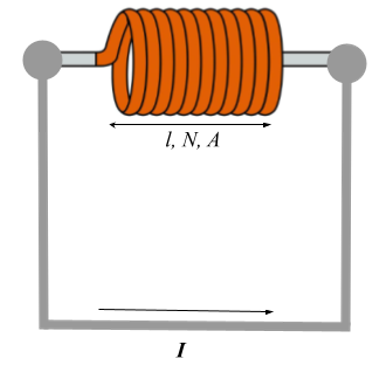
\includegraphics[width=0.3\textwidth]{problems/figures/coilfun.png}
\end{figure*}
\FloatBarrier

\end{problem}
%%\newpage
\begin{problem}{\textbf{\textsc{Coilfun}}}
Xem xét một cuộn dây siêu dẫn không lõi khí với chiều dài \( l = 1 \, \text{m} \), diện tích mặt cắt ngang \( A = 0.1 \, \text{m}^2 \) và số vòng dây \( N = 1000 \). Chúng ta nối hai đầu của cuộn dây với nhau bằng dây siêu dẫn và chạy dòng điện \( I = 1600 \, \text{A} \) qua toàn bộ hệ thống. Giả sử cuộn dây hoạt động lý tưởng.
\newline
\newline
Cosmonaut Carla có một lõi với cùng kích thước như cuộn dây. Lõi có độ từ thẩm tương đối $\frac{\mu_i}{\mu_0} = 10000$ và khối lượng $10\;\mathrm{kg}$. Lõi được thả ở trạng thái nghỉ xa cuộn dây và, do lực từ trường, bay qua cuộn dây. Cosmonaut Carla có thể chọn thời điểm để làm ngừng cuộn dây (ngay lập tức ngắt dòng điện) vào bất kỳ thời điểm nào. Vận tốc thoát tối đa của lõi là bao nhiêu?   


\FloatBarrier
\begin{figure*}[!htbp]
\centering
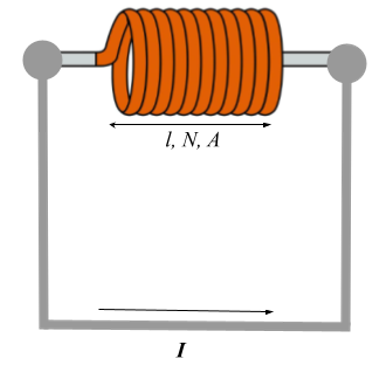
\includegraphics[width=0.3\textwidth]{problems/figures/coilfun.png}
\end{figure*}
\FloatBarrier

\end{problem}

\begin{problem}{\textbf{\textsc{Vào quỹ đạo}}} Một khẩu pháo được cố định trên đỉnh của một mặt phẳng có chiều cao $R = 6.00 \times 10^6\;\mathrm{m}$, mặt phẳng này nằm trên một hành tinh có khối lượng $M = 6.00 \times 10^{24}\;\mathrm{kg}$ và bán kính $R$. Cả khẩu pháo và nền tảng mà nó đặt trên đều có khối lượng không đáng kể. Buồng pháo của khẩu pháo được nghiêng ngang so với hành tinh bên dưới. Khẩu pháo sau đó bắn một quả đạn có khối lượng $m = 45\;\mathrm{kg}$ qua một buồng có chiều dài $l=3\;\mathrm{m}$ với một gia tốc không đổi sao cho quả đạn có thể thành công vào một quỹ đạo elip xung quanh hành tinh. Lực tối thiểu mà khẩu pháo phải áp dụng lên quả đạn để làm điều này là bao nhiêu? Bạn có thể giả định rằng cả hành tinh và mặt phẳng đều không di chuyển trong quá trình này.\end{problem}

\begin{problem}{\textbf{\textsc{Vào quỹ đạo}}} Một khẩu pháo được cố định trên đỉnh của một mặt phẳng có chiều cao $R = 6.00 \times 10^6\;\mathrm{m}$, mặt phẳng này nằm trên một hành tinh có khối lượng $M = 6.00 \times 10^{24}\;\mathrm{kg}$ và bán kính $R$. Cả khẩu pháo và nền tảng mà nó đặt trên đều có khối lượng không đáng kể. Buồng pháo của khẩu pháo được nghiêng ngang so với hành tinh bên dưới. Khẩu pháo sau đó bắn một quả đạn có khối lượng $m = 45\;\mathrm{kg}$ qua một buồng có chiều dài $l=3\;\mathrm{m}$ với một gia tốc không đổi sao cho quả đạn có thể thành công vào một quỹ đạo elip xung quanh hành tinh. Lực tối thiểu mà khẩu pháo phải áp dụng lên quả đạn để làm điều này là bao nhiêu? Bạn có thể giả định rằng cả hành tinh và mặt phẳng đều không di chuyển trong quá trình này.\end{problem}


\begin{problem}
{\textbf{\textsc{Roundabout 1}}} A ramp with length $d$ is raised an angle $\theta$ ($0^{\circ} < \theta < 90^{\circ}$) above the horizontal. A block with mass $m$ is placed at the top of the ramp, with the coefficient of friction between the block and the ramp being $\mu$. Once the block reaches the bottom of the ramp, it retains its velocity as it is smoothly transitioned onto a frictionless circular track with radius $d$ and bank angle $\theta$, rotating on the track without sliding off. A \emph{solution} is a set of values $\{d, \mu, \theta\}$ that result in the situation described above. What is the largest $\theta$ (in degrees) for which a solution exists? 

\end{problem}
\begin{problem}
{\textbf{\textsc{Roundabout 1}}} A ramp with length $d$ is raised an angle $\theta$ ($0^{\circ} < \theta < 90^{\circ}$) above the horizontal. A block with mass $m$ is placed at the top of the ramp, with the coefficient of friction between the block and the ramp being $\mu$. Once the block reaches the bottom of the ramp, it retains its velocity as it is smoothly transitioned onto a frictionless circular track with radius $d$ and bank angle $\theta$, rotating on the track without sliding off. A \emph{solution} is a set of values $\{d, \mu, \theta\}$ that result in the situation described above. What is the largest $\theta$ (in degrees) for which a solution exists? 

\end{problem}

\begin{problem}
{\textbf{\textsc{Roundabout 2}}} Khi khối đi quanh đường tròn, nó được đẩy nhẹ theo phương vuông góc với vận tốc hiện tại của nó và song song với mặt phẳng của đường tròn, gây ra hiện tượng dao động với chu kỳ $T$. Giá trị nhỏ nhất có thể của $T$ khi $d = 5\;\mathrm{m}$ là bao nhiêu?
\end{problem}
\begin{problem}
{\textbf{\textsc{Roundabout 2}}} Khi khối đi quanh đường tròn, nó được đẩy nhẹ theo phương vuông góc với vận tốc hiện tại của nó và song song với mặt phẳng của đường tròn, gây ra hiện tượng dao động với chu kỳ $T$. Giá trị nhỏ nhất có thể của $T$ khi $d = 5\;\mathrm{m}$ là bao nhiêu?
\end{problem}

\begin{problem}{\textbf{\textsc{Đập vỡ nguyên tử}}}
Một hạt alpha là hạt nhân của nguyên tử $^4\text{He}$, và bao gồm hai proton và hai neutron liên kết với nhau. Một neutron được cho vận tốc $v$ và va chạm với một hạt alpha đang đứng yên. Nếu tất cả năm proton và neutron trở nên không liên kết sau va chạm, giá trị nhỏ nhất có thể của $v/c$? là bao nhiêu? Bạn có thể thấy các giá trị sau hữu ích:
$$m_p = 938.27\text{ MeV}/c^2,\quad m_n = 939.57\text{ MeV}/c^2,\quad m_{\alpha} = 3727.4\text{ MeV}/c^2$$
\end{problem}

\begin{problem}{\textbf{\textsc{Đập vỡ nguyên tử}}}
Một hạt alpha là hạt nhân của nguyên tử $^4\text{He}$, và bao gồm hai proton và hai neutron liên kết với nhau. Một neutron được cho vận tốc $v$ và va chạm với một hạt alpha đang đứng yên. Nếu tất cả năm proton và neutron trở nên không liên kết sau va chạm, giá trị nhỏ nhất có thể của $v/c$? là bao nhiêu? Bạn có thể thấy các giá trị sau hữu ích:
$$m_p = 938.27\text{ MeV}/c^2,\quad m_n = 939.57\text{ MeV}/c^2,\quad m_{\alpha} = 3727.4\text{ MeV}/c^2$$
\end{problem}


\begin{problem}{\textbf{\textsc{Tắt đèn}}} 

Follin tạo ra một bể chứa một loại chất lỏng đặc biệt với chỉ số khúc xạ $n = 1 + i(1\cdot 10^{-6}).$ Có vẻ hơi phức tạp. Khi làm việc với chất lỏng này, anh ta vô tình làm rơi một cảm biến ánh sáng vào trong bể. Follin chiếu một tia laser đỏ với bước sóng $\lambda=700\;\text{nm}$ và cường độ trong chân không $I_0 = 5\cdot 10^{6}\;\mathrm{W/m^2}$ xuống chất lỏng. Cảm biến ánh sáng chìm xuống bao xa trước khi phát hiện được cường độ nhỏ hơn $I_f = 10^{-10}\;\mathrm{W/m^2}$? Giả sử rằng phòng thí nghiệm hoàn toàn tối và ánh sáng laser được truyền hoàn toàn vào chất lỏng.  

\end{problem}

\begin{problem}{\textbf{\textsc{Tắt đèn}}} 

Follin tạo ra một bể chứa một loại chất lỏng đặc biệt với chỉ số khúc xạ $n = 1 + i(1\cdot 10^{-6}).$ Có vẻ hơi phức tạp. Khi làm việc với chất lỏng này, anh ta vô tình làm rơi một cảm biến ánh sáng vào trong bể. Follin chiếu một tia laser đỏ với bước sóng $\lambda=700\;\text{nm}$ và cường độ trong chân không $I_0 = 5\cdot 10^{6}\;\mathrm{W/m^2}$ xuống chất lỏng. Cảm biến ánh sáng chìm xuống bao xa trước khi phát hiện được cường độ nhỏ hơn $I_f = 10^{-10}\;\mathrm{W/m^2}$? Giả sử rằng phòng thí nghiệm hoàn toàn tối và ánh sáng laser được truyền hoàn toàn vào chất lỏng.  

\end{problem}


\begin{problem}
\textbf{\textsc{Con lắc cơ giới 1}}
Một con lắc được làm từ một thanh không trọng lượng có chiều dài $l=0.5000\;\mathrm{m}$ và một chất điểm $m=15.00\;\mathrm{kg}$ treo ở một đầu. Góc giữa thanh và phương thẳng đứng là $\theta$. Một động cơ gắn vào điểm xoay cung cấp một mô-men xoắn. Giá trị lớn nhất của moment xoắn này phụ thuộc vào góc và được cho bởi $\tau (\theta)=\frac{1+\cos\theta}{2} \tau_0$ for $0\leq \theta \leq 90^{\circ}$.

\begin{figure}[h]
    \centering
    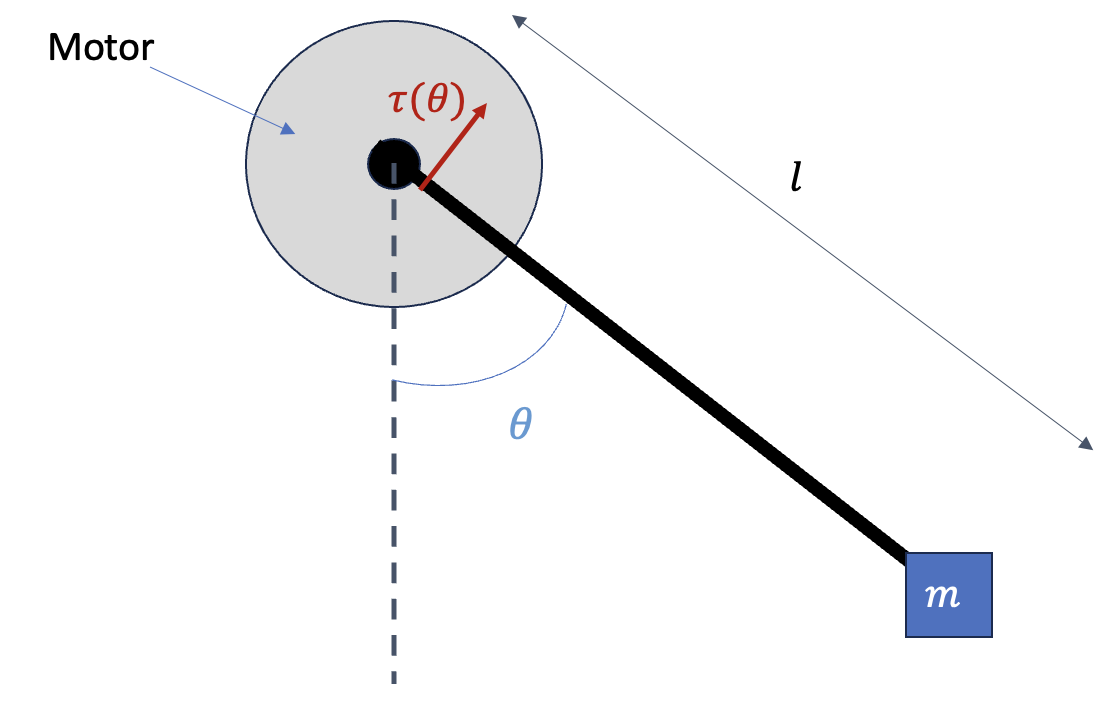
\includegraphics[width=0.5\linewidth]{problems/figures/mot_pend.png}
    \caption{Motorized pendulum}
    \label{fig:enter-label}
\end{figure}

Con lắc ban đầu được cho một vận tốc góc nhỏ theo chiều ngược chiều kim đồng hồ và ở $\theta = 0$. Khối lượng rất nhạy cảm và không thể chịu được tốc độ cao. Do đó, giả sử động cơ luôn cung cấp đủ momemt xoắn để khối lượng di chuyển với tốc độ hầu như không thay đổi. Giá trị nhỏ nhất của $\tau_0$ cần thiết để con lắc cuối cùng đạt đến $\theta=90^{\circ}$ là bao nhiêu?


\end{problem}

\begin{problem}
\textbf{\textsc{Con lắc cơ giới 1}}
Một con lắc được làm từ một thanh không trọng lượng có chiều dài $l=0.5000\;\mathrm{m}$ và một chất điểm $m=15.00\;\mathrm{kg}$ treo ở một đầu. Góc giữa thanh và phương thẳng đứng là $\theta$. Một động cơ gắn vào điểm xoay cung cấp một mô-men xoắn. Giá trị lớn nhất của moment xoắn này phụ thuộc vào góc và được cho bởi $\tau (\theta)=\frac{1+\cos\theta}{2} \tau_0$ for $0\leq \theta \leq 90^{\circ}$.

\begin{figure}[h]
    \centering
    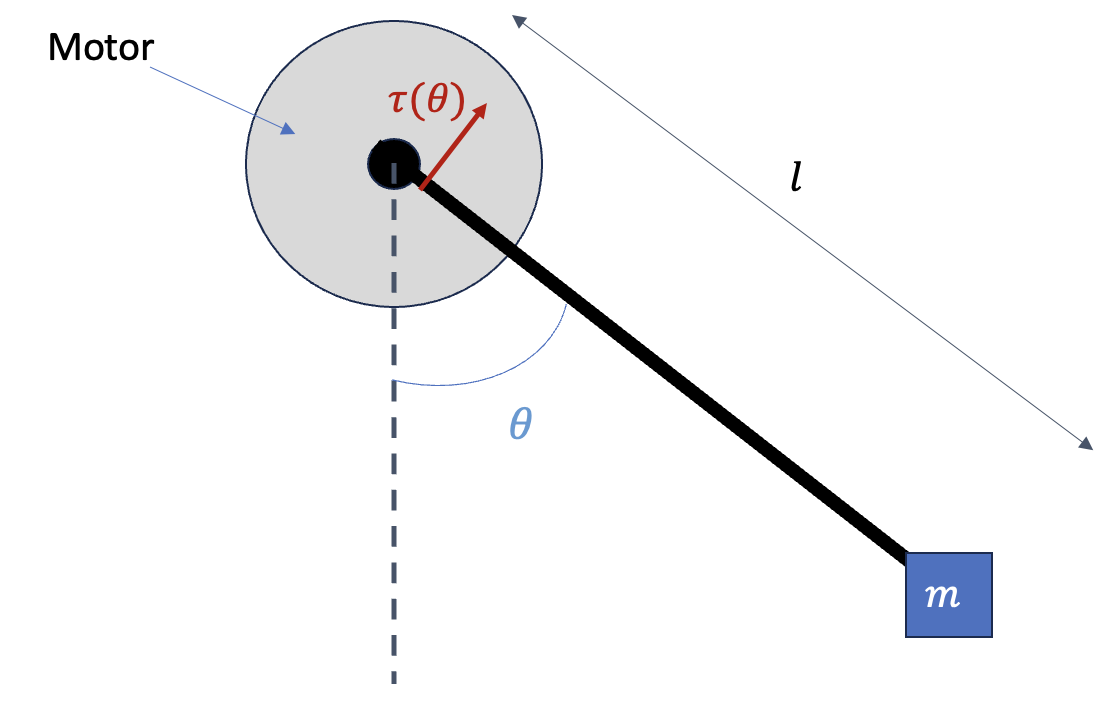
\includegraphics[width=0.5\linewidth]{problems/figures/mot_pend.png}
    \caption{Motorized pendulum}
    \label{fig:enter-label}
\end{figure}

Con lắc ban đầu được cho một vận tốc góc nhỏ theo chiều ngược chiều kim đồng hồ và ở $\theta = 0$. Khối lượng rất nhạy cảm và không thể chịu được tốc độ cao. Do đó, giả sử động cơ luôn cung cấp đủ momemt xoắn để khối lượng di chuyển với tốc độ hầu như không thay đổi. Giá trị nhỏ nhất của $\tau_0$ cần thiết để con lắc cuối cùng đạt đến $\theta=90^{\circ}$ là bao nhiêu?


\end{problem}


\begin{problem}
\textbf{\textsc{Con lắc cơ giới 2}}
Con lắc ban đầu ở $\theta=0$. ần này, khối lượng không còn quá nhạy cảm. Động cơ có thể cung cấp mô-men xoắn tối đa của nó cho tất cả các giá trị của $\theta$. Giá trị nhỏ nhất của $\tau_0$ cần thiết để con lắc đạt đến $\theta=90^{\circ}$ trong một lần dao động đơn chiều là bao nhiêu?    



\end{problem}
    

\begin{problem}
\textbf{\textsc{Con lắc cơ giới 2}}
Con lắc ban đầu ở $\theta=0$. ần này, khối lượng không còn quá nhạy cảm. Động cơ có thể cung cấp mô-men xoắn tối đa của nó cho tất cả các giá trị của $\theta$. Giá trị nhỏ nhất của $\tau_0$ cần thiết để con lắc đạt đến $\theta=90^{\circ}$ trong một lần dao động đơn chiều là bao nhiêu?    



\end{problem}
    


\begin{problem}
\textbf{\textsc{Motorized Pendulum 3}}
The pendulum initially is at $\theta=0$. The mass contains extremely sensitive electronics that cannot tolerate speeds above $v_{max}=0.1000\;\mathrm{m/s}$. To three significant figures, what is the minimum value of $\tau_0$ needed so that the pendulum reaches $\theta=90^{\circ}$ without exceeding this speed threshold?

\end{problem}
\begin{problem}
\textbf{\textsc{Motorized Pendulum 3}}
The pendulum initially is at $\theta=0$. The mass contains extremely sensitive electronics that cannot tolerate speeds above $v_{max}=0.1000\;\mathrm{m/s}$. To three significant figures, what is the minimum value of $\tau_0$ needed so that the pendulum reaches $\theta=90^{\circ}$ without exceeding this speed threshold?

\end{problem}

\begin{problem}
\textbf{\textsc{Dao động hấp dẫn 1}}
%There has been a sad trend in the last decade where more and more people reject basic science and start believing that the earth is flat. While the earth is obviously round, the challenges in making Newtonian gravitation work in a flat world are interesting. So let's have fun at the expense of flat earthers.
Bạn được cung cấp phương trình phân phối điện tích trên một elip dẫn điện được mô tả bởi 
\[
\frac{x^2}{a^2} + \frac{y^2}{b^2} + \frac{z^2}{c^2} = 1
\]
Nếu ta ký hiệu tổng điện tích của nó là \(q\), mật độ điện tích bề mặt \(\sigma\) được cho bởi
\begin{equation*}
\sigma = \frac{q}{4\pi abc} \left( \frac{x^2}{a^4} + \frac{y^2}{b^4} + \frac{z^2}{c^4} \right)^{-1 / 2}
\label{ellipsoidCharge}
\end{equation*}
Giả sử rằng một hành tinh được mô hình hóa như một đĩa có mật độ đồng nhất. Vấn đề với mô hình này là mọi người ở các cạnh sẽ bị kéo về phía trung tâm (chứ không phải "xuống dưới"). Trong trường hợp này, giả sử rằng đĩa có bán kính cố định \(R\) và chiều cao \(h \ll R\). Điều này đi kèm với việc những người khác nhau cảm thấy các "hằng số" hấp dẫn khác nhau theo chiều dọc. Xem xét phân phối mật độ của đĩa \(\rho = \rho(r)\) sao cho mọi người sống trên đó chỉ cảm thấy lực hấp dẫn kéo xuống dưới. Tỷ lệ $\rho(\frac{R}{3})/\rho(\frac{2R}{3})$ là bao nhiêu?

\end{problem}

\begin{problem}
\textbf{\textsc{Dao động hấp dẫn 1}}
%There has been a sad trend in the last decade where more and more people reject basic science and start believing that the earth is flat. While the earth is obviously round, the challenges in making Newtonian gravitation work in a flat world are interesting. So let's have fun at the expense of flat earthers.
Bạn được cung cấp phương trình phân phối điện tích trên một elip dẫn điện được mô tả bởi 
\[
\frac{x^2}{a^2} + \frac{y^2}{b^2} + \frac{z^2}{c^2} = 1
\]
Nếu ta ký hiệu tổng điện tích của nó là \(q\), mật độ điện tích bề mặt \(\sigma\) được cho bởi
\begin{equation*}
\sigma = \frac{q}{4\pi abc} \left( \frac{x^2}{a^4} + \frac{y^2}{b^4} + \frac{z^2}{c^4} \right)^{-1 / 2}
\label{ellipsoidCharge}
\end{equation*}
Giả sử rằng một hành tinh được mô hình hóa như một đĩa có mật độ đồng nhất. Vấn đề với mô hình này là mọi người ở các cạnh sẽ bị kéo về phía trung tâm (chứ không phải "xuống dưới"). Trong trường hợp này, giả sử rằng đĩa có bán kính cố định \(R\) và chiều cao \(h \ll R\). Điều này đi kèm với việc những người khác nhau cảm thấy các "hằng số" hấp dẫn khác nhau theo chiều dọc. Xem xét phân phối mật độ của đĩa \(\rho = \rho(r)\) sao cho mọi người sống trên đó chỉ cảm thấy lực hấp dẫn kéo xuống dưới. Tỷ lệ $\rho(\frac{R}{3})/\rho(\frac{2R}{3})$ là bao nhiêu?

\end{problem}


\begin{solution}

Dựa vào công thức \eqref{densityDistribution} chúng ta có thể thấy rằng
$\rho$ sẽ tiến đến vô cùng khi $r \rightarrow R$. Điều này không thực tế, nên hãy xem liệu việc bỏ qua vòng nhỏ ở bên ngoài có giải quyết được vấn đề này hay không.

\begin{gather*}
    \int^{R}_{R - \epsilon} \rho_0 h \frac{2\pi r \mathrm{d} r}{
    \sqrt{1 - \frac{r ^ 2}{R ^ 2}}} = \pi R ^ 2 h \rho_0 \left.\frac{\left( 1
        - \frac{r^2}{R^2} \right)}{\frac{1}{2}}\right|^R_{R - \epsilon} = \\
     = 2 \pi R h \rho_0 \sqrt{2 R \epsilon} \\
     = 4.12973 \cdot 10 ^ {21} \; \mathrm{kg}
\end{gather*}

\end{solution}
\begin{solution}

Dựa vào công thức \eqref{densityDistribution} chúng ta có thể thấy rằng
$\rho$ sẽ tiến đến vô cùng khi $r \rightarrow R$. Điều này không thực tế, nên hãy xem liệu việc bỏ qua vòng nhỏ ở bên ngoài có giải quyết được vấn đề này hay không.

\begin{gather*}
    \int^{R}_{R - \epsilon} \rho_0 h \frac{2\pi r \mathrm{d} r}{
    \sqrt{1 - \frac{r ^ 2}{R ^ 2}}} = \pi R ^ 2 h \rho_0 \left.\frac{\left( 1
        - \frac{r^2}{R^2} \right)}{\frac{1}{2}}\right|^R_{R - \epsilon} = \\
     = 2 \pi R h \rho_0 \sqrt{2 R \epsilon} \\
     = 4.12973 \cdot 10 ^ {21} \; \mathrm{kg}
\end{gather*}

\end{solution}

\begin{problem}
\textbf{\textsc{Dao động hấp dẫn 3}} 
Giả sử rằng chúng ta khoan một lỗ qua đĩa tại một khoảng cách \(r_0= \frac{R}{3}\) và thả một quả bóng qua lỗ đó. Chu kỳ dao động của quả bóng là bao nhiêu? Bỏ qua lực cản không khí.

\end{problem}

\begin{problem}
\textbf{\textsc{Dao động hấp dẫn 3}} 
Giả sử rằng chúng ta khoan một lỗ qua đĩa tại một khoảng cách \(r_0= \frac{R}{3}\) và thả một quả bóng qua lỗ đó. Chu kỳ dao động của quả bóng là bao nhiêu? Bỏ qua lực cản không khí.

\end{problem}


\begin{solution}
    Bắt đầu bằng cách xem xét một mặt cắt của chất lỏng qua trục trung tâm. Xét một phần khối lượng nhỏ $dm$ của chất lỏng ở bề mặt, cách trục xoay một khoảng $x$ tính từ trục quay. Các lực cân bằng như sau:

$$dN\cos{\theta} = gdm$$

$$dN\sin{\theta} = x\omega^2dm$$

$$\tan{\theta} = \frac{dy}{dx} = \frac{x\omega^2}{g}$$

$$\int dy = \int\frac{x\omega^2}{g}dx\longrightarrow y = \frac{x^2\omega^2}{2g}$$

Phương trình này là parabol, do đó, chất lỏng tạo thành thấu kính dạng paraboloid. Tiêu điểm có thể được tính như sau:

$$f = \bigg(0, \frac{g}{2\omega^2}\bigg)$$

Vì ánh sáng tới theo phương thẳng đứng, photon sẽ va chạm với thấu kính một hoặc hai lần.

Tại mép của giếng trụ, độ cao của chất lỏng so với độ cao tại trung tâm giếng là

$$\frac{\omega^2}{2g}$$

Các điểm tại đó photon tới sẽ va chạm với thấu kính hai lần có thể được tính toán như sau:

$$y = -\bigg(\frac{\omega^2}{2g} - \frac{g}{2\omega^2}\bigg)x + \frac{g}{2\omega^2}$$

$$y = \frac{x^2\omega^2}{2g}$$

$$\frac{g}{2\omega^2} - \frac{x^2\omega^2}{2g} = \bigg(\frac{\omega^2}{2g} - \frac{g}{2\omega^2}\bigg)x$$

$$\frac{x^2\omega^2}{2g} + \bigg(\frac{\omega^2}{2g} - \frac{g}{2\omega^2}\bigg)x - \frac{g}{2\omega^2} = 0$$

$$x = -1, \frac{g^2}{\omega^4}$$

Bất kỳ photon nào ban đầu cách trục trung tâm ít nhất là $\frac{g^2}{\omega^4}$ sẽ va chạm với gương hai lần. Các photon còn lại chỉ va chạm với gương một lần. Giá trị của $n$ có thể được tính như sau.

$$n = 2 - \frac{g^4}{\omega^8} = 2 - \frac{9.8^4}{5^8} \approx \boxed{1.976}$$


\end{solution}
\begin{solution}
    Bắt đầu bằng cách xem xét một mặt cắt của chất lỏng qua trục trung tâm. Xét một phần khối lượng nhỏ $dm$ của chất lỏng ở bề mặt, cách trục xoay một khoảng $x$ tính từ trục quay. Các lực cân bằng như sau:

$$dN\cos{\theta} = gdm$$

$$dN\sin{\theta} = x\omega^2dm$$

$$\tan{\theta} = \frac{dy}{dx} = \frac{x\omega^2}{g}$$

$$\int dy = \int\frac{x\omega^2}{g}dx\longrightarrow y = \frac{x^2\omega^2}{2g}$$

Phương trình này là parabol, do đó, chất lỏng tạo thành thấu kính dạng paraboloid. Tiêu điểm có thể được tính như sau:

$$f = \bigg(0, \frac{g}{2\omega^2}\bigg)$$

Vì ánh sáng tới theo phương thẳng đứng, photon sẽ va chạm với thấu kính một hoặc hai lần.

Tại mép của giếng trụ, độ cao của chất lỏng so với độ cao tại trung tâm giếng là

$$\frac{\omega^2}{2g}$$

Các điểm tại đó photon tới sẽ va chạm với thấu kính hai lần có thể được tính toán như sau:

$$y = -\bigg(\frac{\omega^2}{2g} - \frac{g}{2\omega^2}\bigg)x + \frac{g}{2\omega^2}$$

$$y = \frac{x^2\omega^2}{2g}$$

$$\frac{g}{2\omega^2} - \frac{x^2\omega^2}{2g} = \bigg(\frac{\omega^2}{2g} - \frac{g}{2\omega^2}\bigg)x$$

$$\frac{x^2\omega^2}{2g} + \bigg(\frac{\omega^2}{2g} - \frac{g}{2\omega^2}\bigg)x - \frac{g}{2\omega^2} = 0$$

$$x = -1, \frac{g^2}{\omega^4}$$

Bất kỳ photon nào ban đầu cách trục trung tâm ít nhất là $\frac{g^2}{\omega^4}$ sẽ va chạm với gương hai lần. Các photon còn lại chỉ va chạm với gương một lần. Giá trị của $n$ có thể được tính như sau.

$$n = 2 - \frac{g^4}{\omega^8} = 2 - \frac{9.8^4}{5^8} \approx \boxed{1.976}$$


\end{solution}

\begin{solution}
When the field is active, the pressure $P(x)$ will be exponential because the gas is in hydrostatic equilibrium. Thus, we have $P(x) = P_0 e^{(x-R)\ln(2)/2}$. Because the temperature remains constant, pressure is proportional to density, so $P_1$ will be the average of the initial pressure over the volume of the chamber. Letting $R=1$ and $\displaystyle\frac{\ln(2)}{2} = a$, we have:
\begin{align*}P_{1} &= \frac{3}{4\pi R^3}\iiint_{V}P\ dV\\ &= \frac{3}{4\pi }\int_{-1}^{1}P_{0}e^{a(x-1)}\cdot \pi(1-x^{2})\ dx\\ &= \frac{3P_{0}}{4}\left(e^{a(x-1)}\left(-\frac{x^{2}}{a} + \frac{2x}{a^{2}} + \frac{1}{a} - \frac{2}{a^3}\right)\right)\bigg\vert_{-1}^1\\
&= \frac{3P_0}{4}\left(\left(\frac{2}{a^2}-\frac{2}{a^3}\right)-e^{-2a}\left(-\frac{2}{a^2} -\frac{2}{a^3}\right)\right)\\
&= \boxed{\left(\frac{9}{\ln(2)^{2}} - \frac{6}{\ln(2)^{3}}\right)P_0}\approx 0.716\,P_0\end{align*}
\end{solution}
\begin{solution}
When the field is active, the pressure $P(x)$ will be exponential because the gas is in hydrostatic equilibrium. Thus, we have $P(x) = P_0 e^{(x-R)\ln(2)/2}$. Because the temperature remains constant, pressure is proportional to density, so $P_1$ will be the average of the initial pressure over the volume of the chamber. Letting $R=1$ and $\displaystyle\frac{\ln(2)}{2} = a$, we have:
\begin{align*}P_{1} &= \frac{3}{4\pi R^3}\iiint_{V}P\ dV\\ &= \frac{3}{4\pi }\int_{-1}^{1}P_{0}e^{a(x-1)}\cdot \pi(1-x^{2})\ dx\\ &= \frac{3P_{0}}{4}\left(e^{a(x-1)}\left(-\frac{x^{2}}{a} + \frac{2x}{a^{2}} + \frac{1}{a} - \frac{2}{a^3}\right)\right)\bigg\vert_{-1}^1\\
&= \frac{3P_0}{4}\left(\left(\frac{2}{a^2}-\frac{2}{a^3}\right)-e^{-2a}\left(-\frac{2}{a^2} -\frac{2}{a^3}\right)\right)\\
&= \boxed{\left(\frac{9}{\ln(2)^{2}} - \frac{6}{\ln(2)^{3}}\right)P_0}\approx 0.716\,P_0\end{align*}
\end{solution}

\begin{problem}{\textbf{\textsc{Ping-pong 1}}} A legal serve in ping-pong requires that the ball bounces on one side of the table and that the ball goes over the net. A certain world-class Olympic ping-pong player does the serve at the level of the table at a distance $d=1.37\;\mathrm{m}$ from the net of height $h=15.25\;\mathrm{cm}$. The Olympic player can give the ball such a spin that the translational speed of the ball is conserved after a bounce but the direction of velocity can be controlled freely. What is the minimal serving speed $v_1$ (up to two decimal places)?

\end{problem}
\begin{problem}{\textbf{\textsc{Ping-pong 1}}} A legal serve in ping-pong requires that the ball bounces on one side of the table and that the ball goes over the net. A certain world-class Olympic ping-pong player does the serve at the level of the table at a distance $d=1.37\;\mathrm{m}$ from the net of height $h=15.25\;\mathrm{cm}$. The Olympic player can give the ball such a spin that the translational speed of the ball is conserved after a bounce but the direction of velocity can be controlled freely. What is the minimal serving speed $v_1$ (up to two decimal places)?

\end{problem}

%\begin{problem}{\textbf{\textsc{Ping-pong 2}}} We consider a serve with $n$ bounces before going over the net. The Olympic player is so incredibly good that he can control the direction of the velocity after each bounce as he pleases. Naturally more bounces decreases the minimal serving speed $v_n$. However, for some $N$, when $n\geq N$ the minimal serving speed no longer decreases if bounces are added, i.e. $N$ is the smallest natural number such that $v_m=v_N$ for all $m\geq N.$ Find $v_{N-1}^N$.

%\end{problem}
\begin{problem}{\textbf{\textsc{Ping-pong 2}}} Ta xét một cú giao bóng với $n$ lần nảy trước khi đi qua lưới. Vận động viên Olympic giỏi đến mức anh ấy có thể điều khiển hướng vận tốc sau mỗi lần nảy theo ý muốn. Tất nhiên, nhiều lần nảy hơn sẽ làm giảm tốc độ giao bóng tối thiểu $v_n$. Tuy nhiên, với một số $N$, khi $n\geq N$ tốc độ giao bóng tối thiểu không còn giảm nữa khi thêm lần nảy, nghĩa là $N$ là số tự nhiên nhỏ nhất sao cho $v_m=v_N$ với mọi $m\geq N.$ Tìm $v_{N-1}^N$.
	
\end{problem}
%\begin{problem}{\textbf{\textsc{Ping-pong 2}}} We consider a serve with $n$ bounces before going over the net. The Olympic player is so incredibly good that he can control the direction of the velocity after each bounce as he pleases. Naturally more bounces decreases the minimal serving speed $v_n$. However, for some $N$, when $n\geq N$ the minimal serving speed no longer decreases if bounces are added, i.e. $N$ is the smallest natural number such that $v_m=v_N$ for all $m\geq N.$ Find $v_{N-1}^N$.

%\end{problem}
\begin{problem}{\textbf{\textsc{Ping-pong 2}}} Ta xét một cú giao bóng với $n$ lần nảy trước khi đi qua lưới. Vận động viên Olympic giỏi đến mức anh ấy có thể điều khiển hướng vận tốc sau mỗi lần nảy theo ý muốn. Tất nhiên, nhiều lần nảy hơn sẽ làm giảm tốc độ giao bóng tối thiểu $v_n$. Tuy nhiên, với một số $N$, khi $n\geq N$ tốc độ giao bóng tối thiểu không còn giảm nữa khi thêm lần nảy, nghĩa là $N$ là số tự nhiên nhỏ nhất sao cho $v_m=v_N$ với mọi $m\geq N.$ Tìm $v_{N-1}^N$.
	
\end{problem}

\begin{problem}
{\textbf{\textsc{An Envelope of Light}}} 
A point light source on the ceiling is located at the center of a cylindrical housing (with an open base) of radius $R$ and height $H$. A wall is a horizontal distance $D$ from the center of the cylinder. Now consider a coordinate system with the light source at the origin. The wall, at $x=-D$, has the following shape in the $y-z$ plane:

\begin{center}
    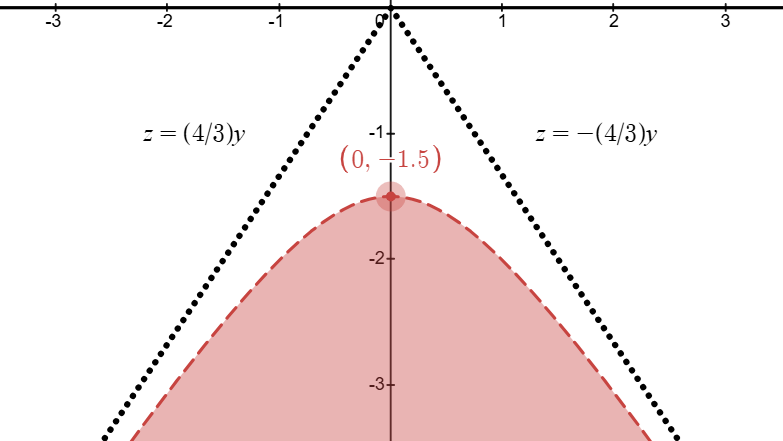
\includegraphics[height=0.3\textwidth]{problems/figures/lightConeGraph.png}
    \hspace{2em}
    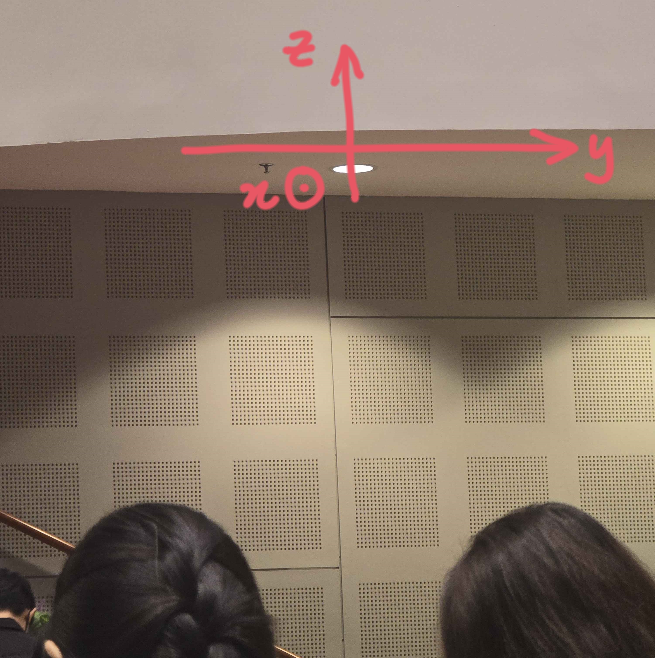
\includegraphics[height=0.3\textwidth]{problems/figures/lightConeHyperbola.png}
\end{center}

The vertical coordinate of the highest point of the curve observed is $-1.5\;\mathrm{m}$, while the gradients of the lines asymptotically tangent to the curve are $\pm 4/3$. On the right is shown an example setup of this phenomenon. Find the horizontal distance $D$ of the wall to the light source.
\end{problem}
\begin{problem}
{\textbf{\textsc{An Envelope of Light}}} 
A point light source on the ceiling is located at the center of a cylindrical housing (with an open base) of radius $R$ and height $H$. A wall is a horizontal distance $D$ from the center of the cylinder. Now consider a coordinate system with the light source at the origin. The wall, at $x=-D$, has the following shape in the $y-z$ plane:

\begin{center}
    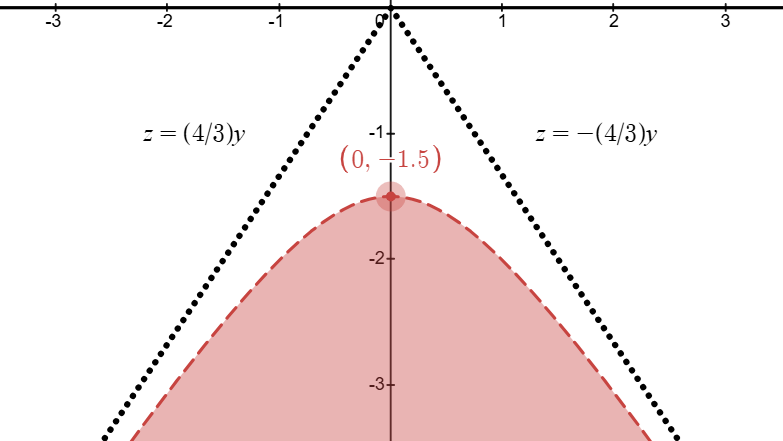
\includegraphics[height=0.3\textwidth]{problems/figures/lightConeGraph.png}
    \hspace{2em}
    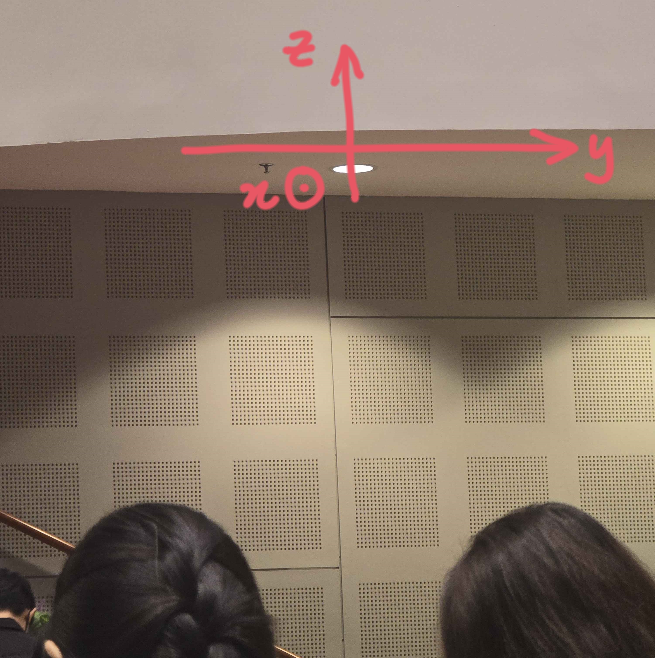
\includegraphics[height=0.3\textwidth]{problems/figures/lightConeHyperbola.png}
\end{center}

The vertical coordinate of the highest point of the curve observed is $-1.5\;\mathrm{m}$, while the gradients of the lines asymptotically tangent to the curve are $\pm 4/3$. On the right is shown an example setup of this phenomenon. Find the horizontal distance $D$ of the wall to the light source.
\end{problem}

\begin{problem}
{\textbf{\textsc{Under The Lamplight}}} A large vat of the magical liquid Ophonium lies before you, with a depth of 5 meters. This liquid has a special property - its index of refraction changes variable to its depth! Its index of refraction can be expressed by the equation $$n = 1 + 2y$$ where $y$ is the depth of the liquid, in meters. A lamp, acting as a point source of light, is hung 3 meters above the vat. Light emanates from the lamp, casting its glow onto a circular section of the Ophonium's surface directly beneath it, covering an area of $3\pi$ square meters. As this light continues to travel downward, it enters the Ophonium, gradually penetrating its depths until it reaches the bottom of the vat. What is the area, in square meters, of the circle illuminated at the bottom of the vat? You may find the following integral useful:
$$\int\frac{1}{\sqrt{x^2-1}}dx = \cosh^{-1}(x) + C$$
\end{problem}
\begin{problem}
{\textbf{\textsc{Under The Lamplight}}} A large vat of the magical liquid Ophonium lies before you, with a depth of 5 meters. This liquid has a special property - its index of refraction changes variable to its depth! Its index of refraction can be expressed by the equation $$n = 1 + 2y$$ where $y$ is the depth of the liquid, in meters. A lamp, acting as a point source of light, is hung 3 meters above the vat. Light emanates from the lamp, casting its glow onto a circular section of the Ophonium's surface directly beneath it, covering an area of $3\pi$ square meters. As this light continues to travel downward, it enters the Ophonium, gradually penetrating its depths until it reaches the bottom of the vat. What is the area, in square meters, of the circle illuminated at the bottom of the vat? You may find the following integral useful:
$$\int\frac{1}{\sqrt{x^2-1}}dx = \cosh^{-1}(x) + C$$
\end{problem}

% \begin{solution}
% Clearly (as $d>h$) if $v$ is high enough, the optimal trajectory to reach $x_{\max}$ is achieved when the launch angle $\alpha=\ang{45}$. Thus we have to first determine whether or not $v$ is high enough.\\

% If $\alpha=\ang{45}$ corresponds to the optimal trajectory over the wall, the highest point of the wall $(d,h)$ is at or under the trajectory. The equation of the trajectory is well-known and easy to derive:
% \[y=-\frac{gx^2}{2v^2\cos^2\alpha}+x\tan\alpha\]
% so $\alpha=\ang{45}$ is optimal if
% \[h\leq -\frac{gd^2}{v^2}+d \implies v\geq d\sqrt{\frac{g}{d-h}}=14\;\mathrm{m/s},\]
% which is not true. Thus $\alpha=\ang{45}$ is not optimal.\\

% Now clearly the ball cannot go over the wall if $\alpha\leq\ang{45}$. Thus we have to increase the angle which decreases the range as the range is a decreasing function of $\alpha$ when $\alpha>\ang{45}$ which can be seen from the range equation (comes directly from the trajectory equation above):
% \[R=\frac{2v^2\sin\alpha\cos\alpha}{g}=\frac{v^2\sin2\alpha}{g}.\]

% Thus the optimal trajectory now is the one that just barely touches the top of the wall for the minimal $\alpha$. I.e. we wish $(d,h)$ to be on the trajectory. If we plug in $(x,y)=(d,h)$ to the trajectory equation and use $1/\cos^2\alpha=1+\tan^2\alpha$ and solve for $\xi\equiv\tan\alpha$ from the quadratic equation that ensues we get two possible roots
% \[\xi_{\pm}=\frac{v^2}{gd}\pm\sqrt{\frac{v^4}{g^2d^2}-\frac{2v^2h}{gd^2}-1}.\]
% As $\xi=\tan\alpha$ and $\tan$ is an increasing function (in our range), we are interested in the smaller root. Thus
% \[\alpha=\arctan{\xi_-}.\]
% Thus the range equation gives us
% \[x_{\max}=\frac{2\xi_-}{1+\xi_-^2}\frac{v^2}{g}.\]

% The argument for the minimal distance is essentially the same. The top of the wall still has to be under the trajectory and $\alpha>\ang{45}$ so now we want the maximal $\alpha$ which corresponds to $\xi_+.$ Thus
% \[x_{\min}=\frac{2\xi_+}{1+\xi_+^2}\frac{v^2}{g}.\]
% And hence
% \[x_{\max}-x_{\min}=\frac{2v^2}{g}\left(\frac{\xi_-}{1+\xi_-^2}-\frac{\xi_+}{1+\xi_+^2}\right)\approx\boxed{5.38\;\mathrm{m}}.\]

% Note for a full solution (not necessary to get the numerical answer) one should also check if the launch speed given is even high enough to go over the wall at all. This minimal speed is relatively easy to derive (especially using the envelope curve):
% \[v_{\min}=\sqrt{gh+g\sqrt{h^2+d^2}}\approx{12.6}\;\mathrm{m/s}<v,\]
% so the question is well-posed.
% \end{solution}

\begin{solution}
Rõ ràng (vì $d>h$) nếu $v$ đủ lớn, quỹ đạo tối ưu để đạt $x_{\max}$ đạt được khi góc phóng $\alpha=\ang{45}$. Do đó, chúng ta phải xác định trước liệu $v$ có đủ lớn hay không.\\

Nếu $\alpha=\ang{45}$ tương ứng với quỹ đạo tối ưu qua tường, điểm cao nhất của tường $(d,h)$ nằm trên hoặc dưới quỹ đạo. Phương trình của quỹ đạo đã được biết đến và dễ dàng suy ra:
\[y=-\frac{gx^2}{2v^2\cos^2\alpha}+x\tan\alpha\]
vì vậy $\alpha=\ang{45}$ là tối ưu nếu
\[h\leq -\frac{gd^2}{v^2}+d \implies v\geq d\sqrt{\frac{g}{d-h}}=14\;\mathrm{m/s},\]
điều này không đúng. Do đó $\alpha=\ang{45}$ không phải là tối ưu.\\

Bây giờ rõ ràng quả bóng không thể vượt qua tường nếu $\alpha\leq\ang{45}$. Do đó, chúng ta phải tăng góc phóng, điều này làm giảm tầm xa vì tầm xa là một hàm giảm của $\alpha$ khi $\alpha>\ang{45}$, điều này có thể thấy từ phương trình tầm xa (trực tiếp từ phương trình quỹ đạo ở trên):
\[R=\frac{2v^2\sin\alpha\cos\alpha}{g}=\frac{v^2\sin2\alpha}{g}.\]

Do đó, quỹ đạo tối ưu bây giờ là quỹ đạo chỉ vừa chạm đỉnh của tường với $\alpha$ nhỏ nhất. Tức là chúng ta muốn $(d,h)$ nằm trên quỹ đạo. Nếu chúng ta thay $(x,y)=(d,h)$ vào phương trình quỹ đạo và sử dụng $1/\cos^2\alpha=1+\tan^2\alpha$ và giải cho $\xi\equiv\tan\alpha$ từ phương trình bậc hai, chúng ta có hai nghiệm khả dĩ
\[\xi_{\pm}=\frac{v^2}{gd}\pm\sqrt{\frac{v^4}{g^2d^2}-\frac{2v^2h}{gd^2}-1}.\]
Vì $\xi=\tan\alpha$ và $\tan$ là một hàm tăng (trong phạm vi của chúng ta), chúng ta quan tâm đến nghiệm nhỏ hơn. Do đó
\[\alpha=\arctan{\xi_-}.\]
Do đó, phương trình tầm xa cho chúng ta
\[x_{\max}=\frac{2\xi_-}{1+\xi_-^2}\frac{v^2}{g}.\]

Lập luận cho khoảng cách tối thiểu về cơ bản là giống nhau. Đỉnh của tường vẫn phải nằm dưới quỹ đạo và $\alpha>\ang{45}$ nên bây giờ chúng ta muốn $\alpha$ lớn nhất tương ứng với $\xi_+.$ Do đó
\[x_{\min}=\frac{2\xi_+}{1+\xi_+^2}\frac{v^2}{g}.\]
Và do đó
\[x_{\max}-x_{\min}=\frac{2v^2}{g}\left(\frac{\xi_-}{1+\xi_-^2}-\frac{\xi_+}{1+\xi_+^2}\right)\approx\boxed{5.38\;\mathrm{m}}.\]

Lưu ý để có một giải pháp đầy đủ (không cần thiết để có được câu trả lời số) người ta cũng nên kiểm tra xem vận tốc phóng đã cho có đủ lớn để vượt qua tường hay không. Vận tốc tối thiểu này tương đối dễ suy ra (đặc biệt là sử dụng đường bao):
\[v_{\min}=\sqrt{gh+g\sqrt{h^2+d^2}}\approx{12.6}\;\mathrm{m/s}<v,\]
vì vậy câu hỏi được đặt ra là hợp lý.
\end{solution}

% \begin{solution}
% Clearly (as $d>h$) if $v$ is high enough, the optimal trajectory to reach $x_{\max}$ is achieved when the launch angle $\alpha=\ang{45}$. Thus we have to first determine whether or not $v$ is high enough.\\

% If $\alpha=\ang{45}$ corresponds to the optimal trajectory over the wall, the highest point of the wall $(d,h)$ is at or under the trajectory. The equation of the trajectory is well-known and easy to derive:
% \[y=-\frac{gx^2}{2v^2\cos^2\alpha}+x\tan\alpha\]
% so $\alpha=\ang{45}$ is optimal if
% \[h\leq -\frac{gd^2}{v^2}+d \implies v\geq d\sqrt{\frac{g}{d-h}}=14\;\mathrm{m/s},\]
% which is not true. Thus $\alpha=\ang{45}$ is not optimal.\\

% Now clearly the ball cannot go over the wall if $\alpha\leq\ang{45}$. Thus we have to increase the angle which decreases the range as the range is a decreasing function of $\alpha$ when $\alpha>\ang{45}$ which can be seen from the range equation (comes directly from the trajectory equation above):
% \[R=\frac{2v^2\sin\alpha\cos\alpha}{g}=\frac{v^2\sin2\alpha}{g}.\]

% Thus the optimal trajectory now is the one that just barely touches the top of the wall for the minimal $\alpha$. I.e. we wish $(d,h)$ to be on the trajectory. If we plug in $(x,y)=(d,h)$ to the trajectory equation and use $1/\cos^2\alpha=1+\tan^2\alpha$ and solve for $\xi\equiv\tan\alpha$ from the quadratic equation that ensues we get two possible roots
% \[\xi_{\pm}=\frac{v^2}{gd}\pm\sqrt{\frac{v^4}{g^2d^2}-\frac{2v^2h}{gd^2}-1}.\]
% As $\xi=\tan\alpha$ and $\tan$ is an increasing function (in our range), we are interested in the smaller root. Thus
% \[\alpha=\arctan{\xi_-}.\]
% Thus the range equation gives us
% \[x_{\max}=\frac{2\xi_-}{1+\xi_-^2}\frac{v^2}{g}.\]

% The argument for the minimal distance is essentially the same. The top of the wall still has to be under the trajectory and $\alpha>\ang{45}$ so now we want the maximal $\alpha$ which corresponds to $\xi_+.$ Thus
% \[x_{\min}=\frac{2\xi_+}{1+\xi_+^2}\frac{v^2}{g}.\]
% And hence
% \[x_{\max}-x_{\min}=\frac{2v^2}{g}\left(\frac{\xi_-}{1+\xi_-^2}-\frac{\xi_+}{1+\xi_+^2}\right)\approx\boxed{5.38\;\mathrm{m}}.\]

% Note for a full solution (not necessary to get the numerical answer) one should also check if the launch speed given is even high enough to go over the wall at all. This minimal speed is relatively easy to derive (especially using the envelope curve):
% \[v_{\min}=\sqrt{gh+g\sqrt{h^2+d^2}}\approx{12.6}\;\mathrm{m/s}<v,\]
% so the question is well-posed.
% \end{solution}

\begin{solution}
Rõ ràng (vì $d>h$) nếu $v$ đủ lớn, quỹ đạo tối ưu để đạt $x_{\max}$ đạt được khi góc phóng $\alpha=\ang{45}$. Do đó, chúng ta phải xác định trước liệu $v$ có đủ lớn hay không.\\

Nếu $\alpha=\ang{45}$ tương ứng với quỹ đạo tối ưu qua tường, điểm cao nhất của tường $(d,h)$ nằm trên hoặc dưới quỹ đạo. Phương trình của quỹ đạo đã được biết đến và dễ dàng suy ra:
\[y=-\frac{gx^2}{2v^2\cos^2\alpha}+x\tan\alpha\]
vì vậy $\alpha=\ang{45}$ là tối ưu nếu
\[h\leq -\frac{gd^2}{v^2}+d \implies v\geq d\sqrt{\frac{g}{d-h}}=14\;\mathrm{m/s},\]
điều này không đúng. Do đó $\alpha=\ang{45}$ không phải là tối ưu.\\

Bây giờ rõ ràng quả bóng không thể vượt qua tường nếu $\alpha\leq\ang{45}$. Do đó, chúng ta phải tăng góc phóng, điều này làm giảm tầm xa vì tầm xa là một hàm giảm của $\alpha$ khi $\alpha>\ang{45}$, điều này có thể thấy từ phương trình tầm xa (trực tiếp từ phương trình quỹ đạo ở trên):
\[R=\frac{2v^2\sin\alpha\cos\alpha}{g}=\frac{v^2\sin2\alpha}{g}.\]

Do đó, quỹ đạo tối ưu bây giờ là quỹ đạo chỉ vừa chạm đỉnh của tường với $\alpha$ nhỏ nhất. Tức là chúng ta muốn $(d,h)$ nằm trên quỹ đạo. Nếu chúng ta thay $(x,y)=(d,h)$ vào phương trình quỹ đạo và sử dụng $1/\cos^2\alpha=1+\tan^2\alpha$ và giải cho $\xi\equiv\tan\alpha$ từ phương trình bậc hai, chúng ta có hai nghiệm khả dĩ
\[\xi_{\pm}=\frac{v^2}{gd}\pm\sqrt{\frac{v^4}{g^2d^2}-\frac{2v^2h}{gd^2}-1}.\]
Vì $\xi=\tan\alpha$ và $\tan$ là một hàm tăng (trong phạm vi của chúng ta), chúng ta quan tâm đến nghiệm nhỏ hơn. Do đó
\[\alpha=\arctan{\xi_-}.\]
Do đó, phương trình tầm xa cho chúng ta
\[x_{\max}=\frac{2\xi_-}{1+\xi_-^2}\frac{v^2}{g}.\]

Lập luận cho khoảng cách tối thiểu về cơ bản là giống nhau. Đỉnh của tường vẫn phải nằm dưới quỹ đạo và $\alpha>\ang{45}$ nên bây giờ chúng ta muốn $\alpha$ lớn nhất tương ứng với $\xi_+.$ Do đó
\[x_{\min}=\frac{2\xi_+}{1+\xi_+^2}\frac{v^2}{g}.\]
Và do đó
\[x_{\max}-x_{\min}=\frac{2v^2}{g}\left(\frac{\xi_-}{1+\xi_-^2}-\frac{\xi_+}{1+\xi_+^2}\right)\approx\boxed{5.38\;\mathrm{m}}.\]

Lưu ý để có một giải pháp đầy đủ (không cần thiết để có được câu trả lời số) người ta cũng nên kiểm tra xem vận tốc phóng đã cho có đủ lớn để vượt qua tường hay không. Vận tốc tối thiểu này tương đối dễ suy ra (đặc biệt là sử dụng đường bao):
\[v_{\min}=\sqrt{gh+g\sqrt{h^2+d^2}}\approx{12.6}\;\mathrm{m/s}<v,\]
vì vậy câu hỏi được đặt ra là hợp lý.
\end{solution}


\begin{solution}

Orient the sphere so its ends are vertical and align on the $z$ axis. The equipotential surfaces are rings with planes parallel to the $xy$ plane. The ring element at polar angle $\phi$ has length (along direction of current) $rd\phi$ and cross section area $2\pi r\sin\phi\cdot t$ (note that $r\gg t$). Integrating from angle $\phi_i=\frac{0.01}{30}$ to $\phi_f=\pi-\frac{0.01}{30}$, the total resistance of the filament is $$R=\int_{\phi_i}^{\phi_f}\frac{\rho\cdot rd\phi}{2\pi r\sin\phi\cdot t}=\boxed{277\;\Omega}.$$

% https://www.wolframalpha.com/input?i2d=true&i=Integrate%5Bcscx%2C%7Bx%2CDivide%5B0.01%2C30%5D%2Cpi-Divide%5B0.01%2C30%5D%7D%5D

\end{solution}
\begin{solution}

Orient the sphere so its ends are vertical and align on the $z$ axis. The equipotential surfaces are rings with planes parallel to the $xy$ plane. The ring element at polar angle $\phi$ has length (along direction of current) $rd\phi$ and cross section area $2\pi r\sin\phi\cdot t$ (note that $r\gg t$). Integrating from angle $\phi_i=\frac{0.01}{30}$ to $\phi_f=\pi-\frac{0.01}{30}$, the total resistance of the filament is $$R=\int_{\phi_i}^{\phi_f}\frac{\rho\cdot rd\phi}{2\pi r\sin\phi\cdot t}=\boxed{277\;\Omega}.$$

% https://www.wolframalpha.com/input?i2d=true&i=Integrate%5Bcscx%2C%7Bx%2CDivide%5B0.01%2C30%5D%2Cpi-Divide%5B0.01%2C30%5D%7D%5D

\end{solution}

\begin{solution}

Let the two contact points be A and B. We use a superposition argument. Consider the following two scenarios:
\begin{itemize}
    \item Inject current $I$ into A and draw out current $I$ uniformly from the surface of the sphere. The current passing through the shell at polar angle $\phi$ is equal to the current leaving the sphere for all polar angles greater than $\phi$, which is $\frac{1+\cos\phi}{2}I$ by consideration of surface area. Then the current density at $\phi$ is $J=\frac{\frac{1+\cos\phi}{2}I}{2\pi r\sin\phi\cdot t}$. Letting $\phi_i=\frac{0.01}{30}$ and $\phi_f=\frac{\pi}{2}-\frac{0.01}{30}$, the voltage between A and B is $$V=\int \mathbf{E}\cdot d\mathbf{l}=\int_{\phi_i}^{\phi_f}\rho J\cdot rd\phi=\int_{\phi_i}^{\phi_f}\frac{\rho I(1+\cos\phi)}{4\pi t\sin\phi}d\phi.$$
    \item Draw out current $I$ from B and inject current $I$ uniformly into the surface of the sphere. We obtain the same voltage between A and B as in the other scenario.
\end{itemize}
Superposing the two scenarios, we have a current distribution that injects current $I$ into A and draws out current $I$ from B, with voltage difference $2V$ between them. Thus, the effective resistance between A and B is $\frac{2V}{I}=2\int_{\phi_i}^{\phi_f}\frac{\rho (1+\cos\phi)}{4\pi t\sin\phi}d\phi=\boxed{266\;\Omega}$.

\end{solution}
\begin{solution}

Let the two contact points be A and B. We use a superposition argument. Consider the following two scenarios:
\begin{itemize}
    \item Inject current $I$ into A and draw out current $I$ uniformly from the surface of the sphere. The current passing through the shell at polar angle $\phi$ is equal to the current leaving the sphere for all polar angles greater than $\phi$, which is $\frac{1+\cos\phi}{2}I$ by consideration of surface area. Then the current density at $\phi$ is $J=\frac{\frac{1+\cos\phi}{2}I}{2\pi r\sin\phi\cdot t}$. Letting $\phi_i=\frac{0.01}{30}$ and $\phi_f=\frac{\pi}{2}-\frac{0.01}{30}$, the voltage between A and B is $$V=\int \mathbf{E}\cdot d\mathbf{l}=\int_{\phi_i}^{\phi_f}\rho J\cdot rd\phi=\int_{\phi_i}^{\phi_f}\frac{\rho I(1+\cos\phi)}{4\pi t\sin\phi}d\phi.$$
    \item Draw out current $I$ from B and inject current $I$ uniformly into the surface of the sphere. We obtain the same voltage between A and B as in the other scenario.
\end{itemize}
Superposing the two scenarios, we have a current distribution that injects current $I$ into A and draws out current $I$ from B, with voltage difference $2V$ between them. Thus, the effective resistance between A and B is $\frac{2V}{I}=2\int_{\phi_i}^{\phi_f}\frac{\rho (1+\cos\phi)}{4\pi t\sin\phi}d\phi=\boxed{266\;\Omega}$.

\end{solution}

\begin{problem}
{\textbf{\textsc{A Question of Counting}}} A uniform beam of cold neutrons (neutrons have mass $m=1.67\times {10}^{-27}\;\mathrm{kg}$ and speed $v=0.66\;\mathrm{m/s}$) passes through a thin slit of width $d=0.5\;\mathrm{mm}$. A detector, of width $w=3$ cm, is placed a distance $r=15\;\mathrm{m}$ from the slit. Find the percentage of neutrons passing through the slit that are actually recorded by the detector.
\end{problem}
\begin{problem}
{\textbf{\textsc{A Question of Counting}}} A uniform beam of cold neutrons (neutrons have mass $m=1.67\times {10}^{-27}\;\mathrm{kg}$ and speed $v=0.66\;\mathrm{m/s}$) passes through a thin slit of width $d=0.5\;\mathrm{mm}$. A detector, of width $w=3$ cm, is placed a distance $r=15\;\mathrm{m}$ from the slit. Find the percentage of neutrons passing through the slit that are actually recorded by the detector.
\end{problem}

\begin{solution}
Let $N$ be the number of particles in the box as a function of time, and let $T_1$ be the temperature of the box as a function of time. Then effusion gives

\begin{equation}
    \frac{dN}{dt}=\frac{2AN}{V}\sqrt{\frac{k_BT_1}{2\pi m}}
\end{equation}

Typically there would be no factor of $2$ and $\frac{dN}{dt}$ would be negative, but $3$ new particles enter the box from the reservoir every time one leaves from the hole. \\
\\
We also know that energy leaves the box through the hole through the thermal energy of the leaving gas. A similar process happens to the gas entering from the reservoir. It can be shown that the average energy of a particle effusing out of a small hole is $2kT$, and since the particles coming in from the reservoir are also effusing in, this is the average energy of the incoming and outgoing particles. The rate of gas leaving is $\frac{1}{2}\frac{dN}{dt}$ and the rate of gas entering is $\frac{3}{2}\frac{dN}{dt}$, so

\begin{align}
    \frac{d}{dt}\left(\frac{3}{2}Nk_BT_1\right)&=\left(\frac{3}{2}\frac{dN}{dt}\right)(2k_BT_2)-\left(\frac{1}{2}\frac{dN}{dt}\right)(2k_BT_1)
\end{align}
    Simplifying yields 

    \begin{equation}
        \frac{dT_1}{dt}=\frac{1}{N}\frac{dN}{dt}\left(2T_2-
        \frac{5}{3}T_1\right)
    \end{equation}
    Plugging in for dN/dt yields

    \begin{equation}
        \frac{dT_1}{dt}=\frac{A}{V}\sqrt{\frac{k_BT_1}{2\pi m}}\left(4T_2-\frac{10}{3}T_1\right)
    \end{equation}
    Integrating this yields
    \begin{equation}
        t=(0.007524)\frac{V}{A}\sqrt{\frac{2\pi m}{k_B}}
    \end{equation}
    Which, plugging in the numbers, is 0.492 days. 
    
\end{solution}
\begin{solution}
Let $N$ be the number of particles in the box as a function of time, and let $T_1$ be the temperature of the box as a function of time. Then effusion gives

\begin{equation}
    \frac{dN}{dt}=\frac{2AN}{V}\sqrt{\frac{k_BT_1}{2\pi m}}
\end{equation}

Typically there would be no factor of $2$ and $\frac{dN}{dt}$ would be negative, but $3$ new particles enter the box from the reservoir every time one leaves from the hole. \\
\\
We also know that energy leaves the box through the hole through the thermal energy of the leaving gas. A similar process happens to the gas entering from the reservoir. It can be shown that the average energy of a particle effusing out of a small hole is $2kT$, and since the particles coming in from the reservoir are also effusing in, this is the average energy of the incoming and outgoing particles. The rate of gas leaving is $\frac{1}{2}\frac{dN}{dt}$ and the rate of gas entering is $\frac{3}{2}\frac{dN}{dt}$, so

\begin{align}
    \frac{d}{dt}\left(\frac{3}{2}Nk_BT_1\right)&=\left(\frac{3}{2}\frac{dN}{dt}\right)(2k_BT_2)-\left(\frac{1}{2}\frac{dN}{dt}\right)(2k_BT_1)
\end{align}
    Simplifying yields 

    \begin{equation}
        \frac{dT_1}{dt}=\frac{1}{N}\frac{dN}{dt}\left(2T_2-
        \frac{5}{3}T_1\right)
    \end{equation}
    Plugging in for dN/dt yields

    \begin{equation}
        \frac{dT_1}{dt}=\frac{A}{V}\sqrt{\frac{k_BT_1}{2\pi m}}\left(4T_2-\frac{10}{3}T_1\right)
    \end{equation}
    Integrating this yields
    \begin{equation}
        t=(0.007524)\frac{V}{A}\sqrt{\frac{2\pi m}{k_B}}
    \end{equation}
    Which, plugging in the numbers, is 0.492 days. 
    
\end{solution}

\begin{problem}{\textbf{\textsc{Air Cushion}}}
An air cushion is in the shape of a cylinder with length $\ell=10.0\;\mathrm{m}$ and circular cross-sectional radius $R=28\;\mathrm{cm}$. The ends of the cylinder lie in vertical planes, and the length lies parallel to the horizontal ground. It is filled with an incompressible gas. Both the surface of the air cushion and gas inside have negligible weight compared to other forces in the scenario. The surface maintains a a constant surface tension $\gamma=5.0\;\mathrm{N/m}$ whenever deformed. A flat slab of mass $m=12.0\;\mathrm{kg}$ which is wider than the cushion is balanced on top, squishing the cushion. Find the new horizontal width of the cushion. Assume that its cross-section remains symmetric about a vertical axis.

\end{problem}
\begin{problem}{\textbf{\textsc{Air Cushion}}}
An air cushion is in the shape of a cylinder with length $\ell=10.0\;\mathrm{m}$ and circular cross-sectional radius $R=28\;\mathrm{cm}$. The ends of the cylinder lie in vertical planes, and the length lies parallel to the horizontal ground. It is filled with an incompressible gas. Both the surface of the air cushion and gas inside have negligible weight compared to other forces in the scenario. The surface maintains a a constant surface tension $\gamma=5.0\;\mathrm{N/m}$ whenever deformed. A flat slab of mass $m=12.0\;\mathrm{kg}$ which is wider than the cushion is balanced on top, squishing the cushion. Find the new horizontal width of the cushion. Assume that its cross-section remains symmetric about a vertical axis.

\end{problem}

\begin{solution}
Let the angle of the sides change by $\theta$. The kinetic energy can be written as
\[K=4\cdot\frac{1}{2}\left(\frac{1}{12}m\ell^2+m\frac{\ell^2}{4}\right)\dot\theta^2=\frac 23 m\ell^2\dot\theta^2.\]

The potential energy associated with the soap film is simply
\[U_\sigma=2\sigma\ell^2\cos(2\theta)\simeq 2\sigma\ell^2\left(1-2\theta^2\right).\]
The potential energy associated with the positions of the charges is simply
\[U_\varepsilon=\frac{kq^2}{\ell}\left(4+\frac{1}{2\sin\left(\pi/4-\theta\right)}+\frac{1}{2\sin(\pi/4+\theta)}\right)\simeq \frac{kq^2}{\ell}\left(4+\sqrt{2}+\frac{3\sqrt{2}}{2}\theta^2\right).\]

Total energy is conserved and thus $\dot E=0.$ Differentiating the total energy and regrouping the terms thus gives
\[\ddot\theta+\frac{9\sqrt{2}\frac{kq^2}{\ell}-24\sigma\ell^2}{4 m\ell^2}\theta=0.\]
Thus
\[\omega=\sqrt{\frac{9\sqrt{2}\frac{kq^2}{\ell}-24\sigma\ell^2}{4 m\ell^2}}\approx \boxed{1.43\;\mathrm{rad/s}.}\]
\end{solution}
\begin{solution}
Let the angle of the sides change by $\theta$. The kinetic energy can be written as
\[K=4\cdot\frac{1}{2}\left(\frac{1}{12}m\ell^2+m\frac{\ell^2}{4}\right)\dot\theta^2=\frac 23 m\ell^2\dot\theta^2.\]

The potential energy associated with the soap film is simply
\[U_\sigma=2\sigma\ell^2\cos(2\theta)\simeq 2\sigma\ell^2\left(1-2\theta^2\right).\]
The potential energy associated with the positions of the charges is simply
\[U_\varepsilon=\frac{kq^2}{\ell}\left(4+\frac{1}{2\sin\left(\pi/4-\theta\right)}+\frac{1}{2\sin(\pi/4+\theta)}\right)\simeq \frac{kq^2}{\ell}\left(4+\sqrt{2}+\frac{3\sqrt{2}}{2}\theta^2\right).\]

Total energy is conserved and thus $\dot E=0.$ Differentiating the total energy and regrouping the terms thus gives
\[\ddot\theta+\frac{9\sqrt{2}\frac{kq^2}{\ell}-24\sigma\ell^2}{4 m\ell^2}\theta=0.\]
Thus
\[\omega=\sqrt{\frac{9\sqrt{2}\frac{kq^2}{\ell}-24\sigma\ell^2}{4 m\ell^2}}\approx \boxed{1.43\;\mathrm{rad/s}.}\]
\end{solution}



\begin{problem}

\textbf{\textsc{Relativistic Scattering}} A small spherical particle traveling at a speed $v=0.5c$ at an angle $\alpha=45^{\circ}$ from the horizontal is struck by an electromagnetic plane wave of angular frequency $\omega=7.08\times 10^{15} \;\mathrm{Hz}$ propagating directly to the right. In its own reference frame, the particle scatters light in all directions with the same frequency as the frequency of incident light it perceives. Due to the relativistic Doppler effect, however, the frequency of the scattered light measured in the lab frame is generally not the same as the incident light frequency. What is the angular frequency $\omega'$ of light scattered into a scattering angle of $\theta=89^{\circ}$? Assume the radius of the particle $R$ is small enough that $R\omega \ll c$.
\FloatBarrier
\begin{figure}[h]
    \centering
    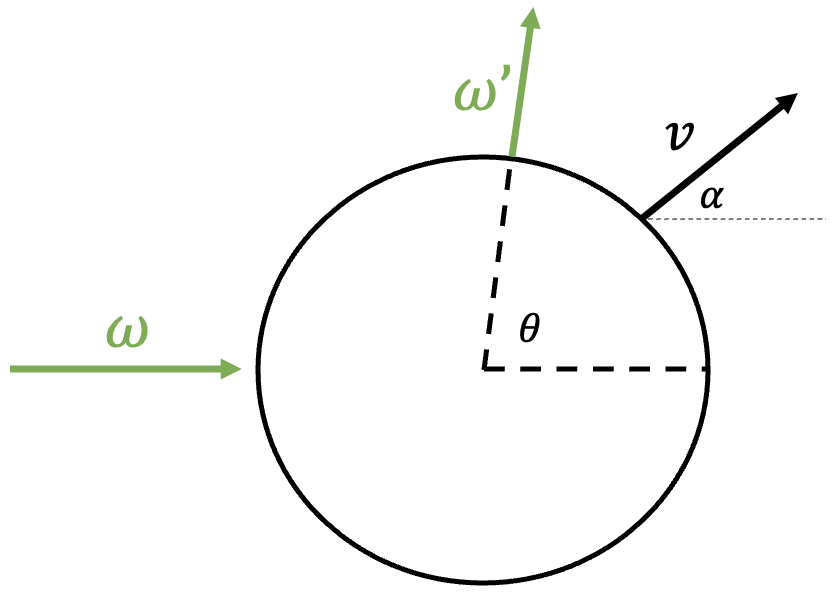
\includegraphics[width=0.4\linewidth]{problems/figures/rel_sca_fig.png}
    % \caption{Setup. Pictured is the scattering angle $\theta$ and the velocity $v$ of the particle. Contrary to what the coloring would suggest, the scattered light frequency $\omega'$ might not be the same as the incident light frequency $\omega$.}
    \label{fig:enter-label}
\end{figure}
\FloatBarrier
\end{problem}



\begin{problem}

\textbf{\textsc{Relativistic Scattering}} A small spherical particle traveling at a speed $v=0.5c$ at an angle $\alpha=45^{\circ}$ from the horizontal is struck by an electromagnetic plane wave of angular frequency $\omega=7.08\times 10^{15} \;\mathrm{Hz}$ propagating directly to the right. In its own reference frame, the particle scatters light in all directions with the same frequency as the frequency of incident light it perceives. Due to the relativistic Doppler effect, however, the frequency of the scattered light measured in the lab frame is generally not the same as the incident light frequency. What is the angular frequency $\omega'$ of light scattered into a scattering angle of $\theta=89^{\circ}$? Assume the radius of the particle $R$ is small enough that $R\omega \ll c$.
\FloatBarrier
\begin{figure}[h]
    \centering
    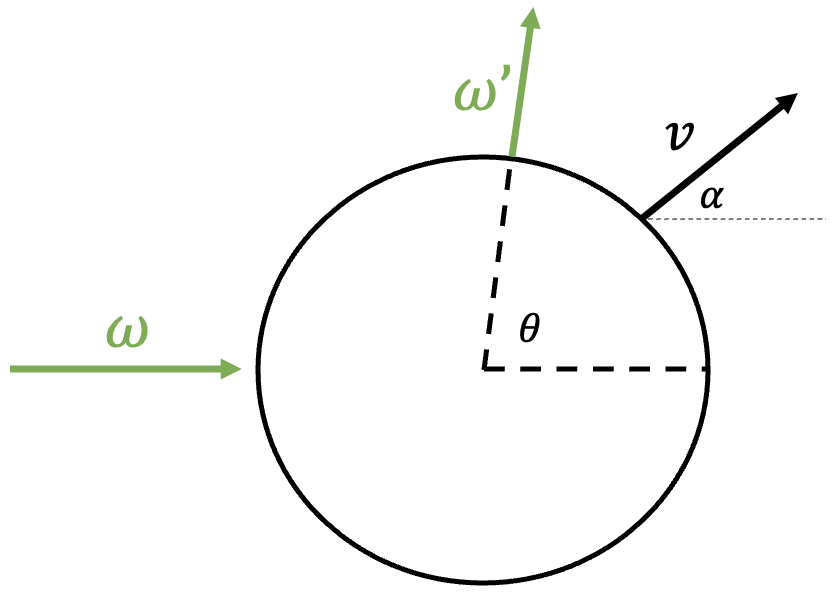
\includegraphics[width=0.4\linewidth]{problems/figures/rel_sca_fig.png}
    % \caption{Setup. Pictured is the scattering angle $\theta$ and the velocity $v$ of the particle. Contrary to what the coloring would suggest, the scattered light frequency $\omega'$ might not be the same as the incident light frequency $\omega$.}
    \label{fig:enter-label}
\end{figure}
\FloatBarrier
\end{problem}


\begin{solution}
The motion can be divided into two regimes: rolling-without slipping, where the frictional force is large enough to counteract the tension, and rolling-with-slipping, which slows the rotation until $\theta$ reaches a maximum. First, let's consider the period where the hoop rolls without slipping. If $F_f$ is the magnitude of the frictional force, we have:
$$\ddot{x} = r\ddot{\theta} \Longrightarrow \frac{T - F_f}{m} = \frac{Tr\cos\theta + F_f r}{mr^2}\Longrightarrow F_f = \frac{T(1-\cos\theta)}{2}$$
Because $F_f\leq\mu mg$, rolling without slipping ends at the critical angle $\displaystyle\theta_c = \cos^{-1}\left(1 - \frac{2\mu mg}{T}\right)$. To fully define the initial conditions, we must also find $\dot{\theta}$ at the critical point. Consider the equation of motion for $\theta$ during rolling-without-slipping:
$$\ddot{\theta} = \dot{\theta}\,\frac{d\dot{\theta}}{d\theta}= \frac{Tr\cos\theta + F_f r}{mr^2} = \frac{T(1+\cos\theta)}{2mr}$$
$$\Rightarrow \int_{0}^{\theta_c}\dot{\theta}\ d\dot{\theta} = \int_0^{\theta_c}\frac{T(1+\cos(\theta))}{2mr}\ d\theta\Rightarrow \dot{\theta}_c^2 = \frac{T(\theta_c +\sin(\theta_c))}{mr}$$

Now, consider the rolling-with-slipping period. Letting $\theta_m$ be the maximum value of $\theta$ reached, we will use the same trick to compute $\dot{\theta}_m$:
$$\ddot{\theta} = \dot{\theta}\,\frac{d\dot{\theta}}{d\theta}= \frac{Tr\cos\theta + F_f r}{mr^2} = \frac{T\cos(\theta)}{mr} + \frac{\mu g}{r}$$
$$\Rightarrow \int_{\theta_c}^{\theta_m}\dot{\theta}\ d\dot{\theta} = \int_{\theta_c}^{\theta_m}\frac{T\cos(\theta)}{mr} + \frac{\mu g}{r}\ d\theta\Rightarrow \frac{\dot{\theta}_{m}^2}{2} - \frac{\dot{\theta}^2_c}{2} = \frac{\mu g(\theta_m - \theta_c)}{r} + \frac{T(\sin(\theta_m) - \sin(\theta_c))}{mr}$$
$$\Rightarrow \dot{\theta}_{m}^2 =  \frac{2\mu g(\theta_m - \theta_c)}{r} + \frac{T(2\sin(\theta_m) + \theta_c-\sin(\theta_c))}{mr}$$
For the hoop to stop at $\theta_m$, we must have $\dot{\theta}_{m} = 0$. Thus:
$$\frac{mr}{T}\dot{\theta}_{m}^2 = \frac{2\mu mg(\theta_m-\theta_c)}{T} + 2\sin(\theta_m) +\theta_c - \sin(\theta_c) = 0$$
Letting $\displaystyle a = \frac{T}{\mu mg}$:
$$\Rightarrow \frac{2(\theta_m - \cos^{-1}(1 - 2/a))}{a} + 2\sin(\theta_m) + \cos^{-1}(1-2/a) - \sin(\cos^{-1}(1 - 2/a)) = 0$$
$$\Rightarrow \theta_m + a\sin(\theta_m) + (a/2 - 1)\cos^{-1}(1-2/a) - \sqrt{a-1} = 0$$
Next, we graph this implicit function of $\theta_m$ and $a$ (taking care to limit ourselves to the physically relevant region where $\theta_m > \theta_c$). We find that the minimum value of $a$ over all solutions is $\boxed{3.888}$. The equivalent condition $\displaystyle\frac{da}{d\theta_m}=0$ can be used to find the solution without graphing.
\end{solution}
\begin{solution}
The motion can be divided into two regimes: rolling-without slipping, where the frictional force is large enough to counteract the tension, and rolling-with-slipping, which slows the rotation until $\theta$ reaches a maximum. First, let's consider the period where the hoop rolls without slipping. If $F_f$ is the magnitude of the frictional force, we have:
$$\ddot{x} = r\ddot{\theta} \Longrightarrow \frac{T - F_f}{m} = \frac{Tr\cos\theta + F_f r}{mr^2}\Longrightarrow F_f = \frac{T(1-\cos\theta)}{2}$$
Because $F_f\leq\mu mg$, rolling without slipping ends at the critical angle $\displaystyle\theta_c = \cos^{-1}\left(1 - \frac{2\mu mg}{T}\right)$. To fully define the initial conditions, we must also find $\dot{\theta}$ at the critical point. Consider the equation of motion for $\theta$ during rolling-without-slipping:
$$\ddot{\theta} = \dot{\theta}\,\frac{d\dot{\theta}}{d\theta}= \frac{Tr\cos\theta + F_f r}{mr^2} = \frac{T(1+\cos\theta)}{2mr}$$
$$\Rightarrow \int_{0}^{\theta_c}\dot{\theta}\ d\dot{\theta} = \int_0^{\theta_c}\frac{T(1+\cos(\theta))}{2mr}\ d\theta\Rightarrow \dot{\theta}_c^2 = \frac{T(\theta_c +\sin(\theta_c))}{mr}$$

Now, consider the rolling-with-slipping period. Letting $\theta_m$ be the maximum value of $\theta$ reached, we will use the same trick to compute $\dot{\theta}_m$:
$$\ddot{\theta} = \dot{\theta}\,\frac{d\dot{\theta}}{d\theta}= \frac{Tr\cos\theta + F_f r}{mr^2} = \frac{T\cos(\theta)}{mr} + \frac{\mu g}{r}$$
$$\Rightarrow \int_{\theta_c}^{\theta_m}\dot{\theta}\ d\dot{\theta} = \int_{\theta_c}^{\theta_m}\frac{T\cos(\theta)}{mr} + \frac{\mu g}{r}\ d\theta\Rightarrow \frac{\dot{\theta}_{m}^2}{2} - \frac{\dot{\theta}^2_c}{2} = \frac{\mu g(\theta_m - \theta_c)}{r} + \frac{T(\sin(\theta_m) - \sin(\theta_c))}{mr}$$
$$\Rightarrow \dot{\theta}_{m}^2 =  \frac{2\mu g(\theta_m - \theta_c)}{r} + \frac{T(2\sin(\theta_m) + \theta_c-\sin(\theta_c))}{mr}$$
For the hoop to stop at $\theta_m$, we must have $\dot{\theta}_{m} = 0$. Thus:
$$\frac{mr}{T}\dot{\theta}_{m}^2 = \frac{2\mu mg(\theta_m-\theta_c)}{T} + 2\sin(\theta_m) +\theta_c - \sin(\theta_c) = 0$$
Letting $\displaystyle a = \frac{T}{\mu mg}$:
$$\Rightarrow \frac{2(\theta_m - \cos^{-1}(1 - 2/a))}{a} + 2\sin(\theta_m) + \cos^{-1}(1-2/a) - \sin(\cos^{-1}(1 - 2/a)) = 0$$
$$\Rightarrow \theta_m + a\sin(\theta_m) + (a/2 - 1)\cos^{-1}(1-2/a) - \sqrt{a-1} = 0$$
Next, we graph this implicit function of $\theta_m$ and $a$ (taking care to limit ourselves to the physically relevant region where $\theta_m > \theta_c$). We find that the minimum value of $a$ over all solutions is $\boxed{3.888}$. The equivalent condition $\displaystyle\frac{da}{d\theta_m}=0$ can be used to find the solution without graphing.
\end{solution}

%\begin{problem}{\textbf{\textsc{Solenoid Spring}}\hspace{1mm}}
%A solenoid also functions as a spring of spring constant $k=50\;\mathrm{N/m}$. It is connected in series with a resistor of very small resistance. One end of the solenoid is firmly fixed to its wire while the other end has a conducting ring of mass $m=0.25\;\mathrm{kg}$ that is free to frictionlessly slide on its wire but always remains in contact. The inductance is $L_0=3.0\;\mathrm{mH}$ at its relaxed length $\ell_0=20\;\mathrm{cm}$. If the free end of the solenoid is slightly displaced, find the angular frequency of the resulting oscillations. The initial current through the circuit is $I=8\;\mathrm{A}$. Assume that the thermal power lost by the resistor is negligible.
%\end{problem}

\begin{problem}{\textbf{\textsc{Solenoid Spring}}\hspace{1mm}}
	Một cuộn cảm dài cũng hoạt động như một lò xo với độ cứng $k=50\;\mathrm{N/m}$. Cuộn cảm này được kết nối với một điện trở có điện trở rất nhỏ. Một đầu của cuộn cảm được gắn cố định vào dây, trong khi đầu còn lại có một vòng dẫn điện có khối lượng $m=0.25\;\mathrm{kg}$ có thể trượt mà không ma sát trên dây nhưng luôn tiếp xúc. Độ tự cảm của cuộn dây là $L_0=3.0\;\mathrm{mH}$ ở chiều dài tự nhiên $\ell_0=20\;\mathrm{cm}$. Nếu đầu tự do của cuộn dây bị dịch chuyển nhẹ, hãy tìm tần số góc của các dao động phát sinh. Dòng điện ban đầu qua mạch là $I=8\;\mathrm{A}$. Giả sử rằng công suất nhiệt mất mát bởi điện trở là không đáng kể.    
\end{problem}
%\begin{problem}{\textbf{\textsc{Solenoid Spring}}\hspace{1mm}}
%A solenoid also functions as a spring of spring constant $k=50\;\mathrm{N/m}$. It is connected in series with a resistor of very small resistance. One end of the solenoid is firmly fixed to its wire while the other end has a conducting ring of mass $m=0.25\;\mathrm{kg}$ that is free to frictionlessly slide on its wire but always remains in contact. The inductance is $L_0=3.0\;\mathrm{mH}$ at its relaxed length $\ell_0=20\;\mathrm{cm}$. If the free end of the solenoid is slightly displaced, find the angular frequency of the resulting oscillations. The initial current through the circuit is $I=8\;\mathrm{A}$. Assume that the thermal power lost by the resistor is negligible.
%\end{problem}

\begin{problem}{\textbf{\textsc{Solenoid Spring}}\hspace{1mm}}
	Một cuộn cảm dài cũng hoạt động như một lò xo với độ cứng $k=50\;\mathrm{N/m}$. Cuộn cảm này được kết nối với một điện trở có điện trở rất nhỏ. Một đầu của cuộn cảm được gắn cố định vào dây, trong khi đầu còn lại có một vòng dẫn điện có khối lượng $m=0.25\;\mathrm{kg}$ có thể trượt mà không ma sát trên dây nhưng luôn tiếp xúc. Độ tự cảm của cuộn dây là $L_0=3.0\;\mathrm{mH}$ ở chiều dài tự nhiên $\ell_0=20\;\mathrm{cm}$. Nếu đầu tự do của cuộn dây bị dịch chuyển nhẹ, hãy tìm tần số góc của các dao động phát sinh. Dòng điện ban đầu qua mạch là $I=8\;\mathrm{A}$. Giả sử rằng công suất nhiệt mất mát bởi điện trở là không đáng kể.    
\end{problem}

%\begin{problem}{\textbf{\textsc{Devil's Trill}}}
%Consider a string of length $L=1\;\mathrm{m}$ and linear mass density $\lambda$\ =\ 1\ g/m, fixed on both ends and vibrating in the first normal mode with amplitude $A = 0.125 \; \mathrm{cm}$. A frictionless, negligibly-small finger, initially at the right endpoint, slides slowly toward the left, flattening the oscillation as it goes. When the vibrating part of the string has length $L_2=12.5\;\mathrm{cm}$, find the new amplitude of vibrations $A_2$, in meters. You may assume $A_2\ll L_2$. Diagrams are not necessarily drawn to scale. 

%\FloatBarrier
%\begin{figure*}[!htbp]
%\centering
%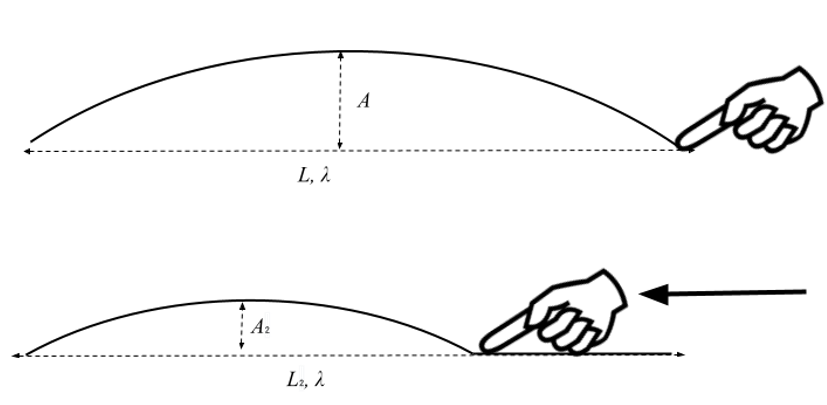
\includegraphics[width=0.6\textwidth]{problems/figures/devilTrill.png}
%\end{figure*}
%\FloatBarrier



%\end{problem}

\begin{problem}{\textbf{\textsc{Devil's Trill}}}
	Xem xét một sợi dây có chiều dài $L=1\;\mathrm{m}$ và mật độ khối lượng tuyến tính $\lambda$\ =\ 1\ g/m, được cố định ở cả hai đầu và dao động ở chế độ dao động chuẩn thứ nhất với biên độ $A = 0.125 \; \mathrm{cm}$. Một ngón tay không ma sát, có kích thước không đáng kể, ban đầu ở điểm cuối bên phải, trượt chậm về phía bên trái, làm phẳng dao động khi nó di chuyển. Khi phần dao động của sợi dây có chiều dài $L_2=12.5\;\mathrm{cm}$, hãy tìm biên độ dao động mới $A_2$, ở đơn vị mét. Bạn có thể giả sử rằng $A_2\ll L_2$. Các hình vẽ không nhất thiết phải được vẽ theo tỷ lệ. 
	
	\FloatBarrier
	\begin{figure*}[!htbp]
		\centering
		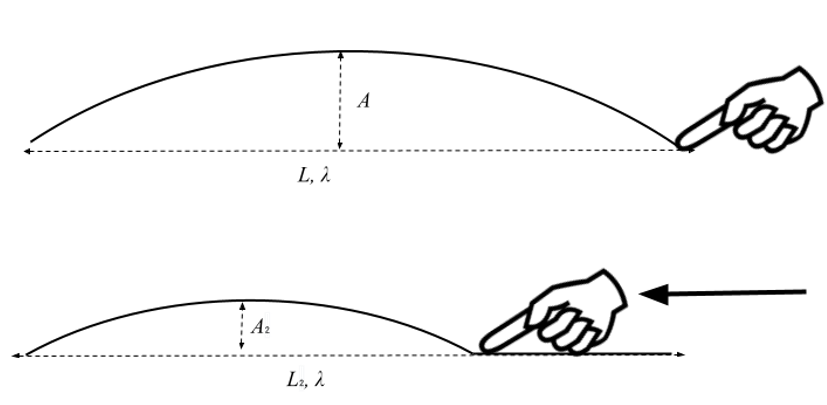
\includegraphics[width=0.6\textwidth]{problems/figures/devilTrill.png}
	\end{figure*}
	\FloatBarrier
	
	
	
\end{problem}
%\begin{problem}{\textbf{\textsc{Devil's Trill}}}
%Consider a string of length $L=1\;\mathrm{m}$ and linear mass density $\lambda$\ =\ 1\ g/m, fixed on both ends and vibrating in the first normal mode with amplitude $A = 0.125 \; \mathrm{cm}$. A frictionless, negligibly-small finger, initially at the right endpoint, slides slowly toward the left, flattening the oscillation as it goes. When the vibrating part of the string has length $L_2=12.5\;\mathrm{cm}$, find the new amplitude of vibrations $A_2$, in meters. You may assume $A_2\ll L_2$. Diagrams are not necessarily drawn to scale. 

%\FloatBarrier
%\begin{figure*}[!htbp]
%\centering
%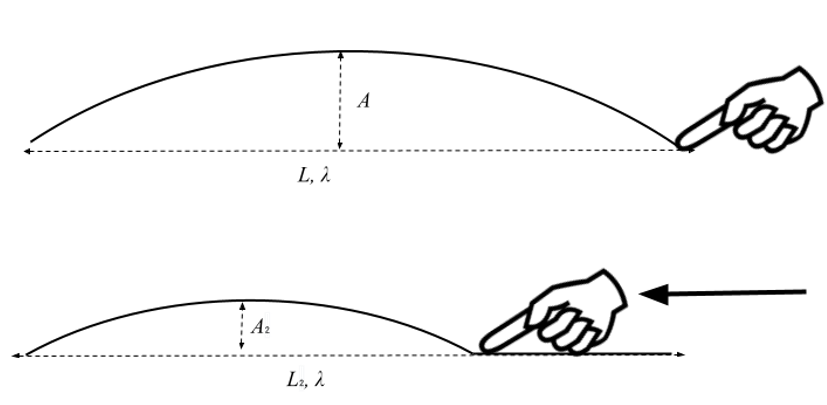
\includegraphics[width=0.6\textwidth]{problems/figures/devilTrill.png}
%\end{figure*}
%\FloatBarrier



%\end{problem}

\begin{problem}{\textbf{\textsc{Devil's Trill}}}
	Xem xét một sợi dây có chiều dài $L=1\;\mathrm{m}$ và mật độ khối lượng tuyến tính $\lambda$\ =\ 1\ g/m, được cố định ở cả hai đầu và dao động ở chế độ dao động chuẩn thứ nhất với biên độ $A = 0.125 \; \mathrm{cm}$. Một ngón tay không ma sát, có kích thước không đáng kể, ban đầu ở điểm cuối bên phải, trượt chậm về phía bên trái, làm phẳng dao động khi nó di chuyển. Khi phần dao động của sợi dây có chiều dài $L_2=12.5\;\mathrm{cm}$, hãy tìm biên độ dao động mới $A_2$, ở đơn vị mét. Bạn có thể giả sử rằng $A_2\ll L_2$. Các hình vẽ không nhất thiết phải được vẽ theo tỷ lệ. 
	
	\FloatBarrier
	\begin{figure*}[!htbp]
		\centering
		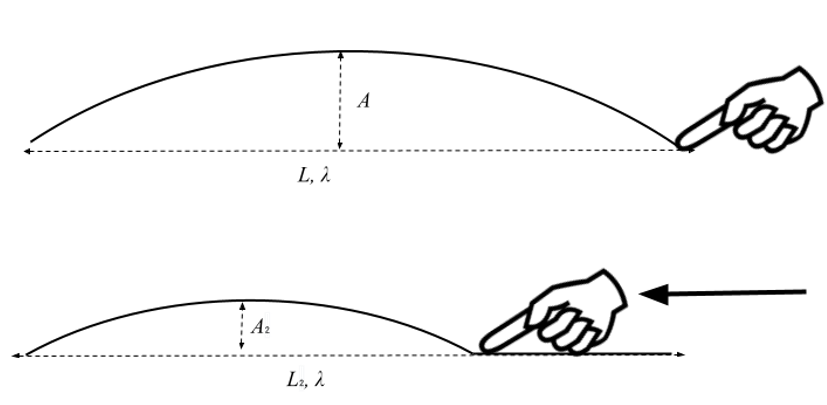
\includegraphics[width=0.6\textwidth]{problems/figures/devilTrill.png}
	\end{figure*}
	\FloatBarrier
	
	
	
\end{problem}

\begin{problem}{\textbf{\textsc{Chess}}}
%Proposed rewording (by Eppu):
Imagine a $4 \times 4$ grid with a particle in each cell. These particles move in an L-shape, similar to knights in chess. Every second, a particle moves randomly in one of the cells it can access with an L jump. Two or more particles are allowed to occupy the same cell. After some time, this system will reach an equilibrium. If the (statistical) temperature of the system and thus each cell is $T=1\; \mathrm{mK}$, all the cells will have a definite energy level. Find the difference between the highest and lowest energy states in $\mathrm{eV}$.

%Imagine a $4 \times 4$ lattice with a particle in each cell. These particles move in an L-shape,
%similar to knights in chess. Every second, a particle moves randomly in one of the cells it
%can access with an L jump. Two or more particles are allowed to occupy the same cell. After some time, this system will reach an equilibrium. 

% Let $A,B,C,D$ be the expected number of particles in each cell of the second row.  Find $p+q$, where $p,q$ are relatively prime positive integers such that $\frac{p}{q}=A\cdot B\cdot C\cdot D$.

%We can assign an energy to each cell based on the probability of a particle begin there. Consider $T = 1\;\mathrm{mK}$ given. Find the difference between the smallest and the largest equivalent energies in $eV$.

%For a harder problem, try it on an $n \times n$ lattice. If this is easy too switch to queen-like moves and try get a closed form formula. (may be a bit more mathematical)



\end{problem}
\begin{problem}{\textbf{\textsc{Chess}}}
%Proposed rewording (by Eppu):
Imagine a $4 \times 4$ grid with a particle in each cell. These particles move in an L-shape, similar to knights in chess. Every second, a particle moves randomly in one of the cells it can access with an L jump. Two or more particles are allowed to occupy the same cell. After some time, this system will reach an equilibrium. If the (statistical) temperature of the system and thus each cell is $T=1\; \mathrm{mK}$, all the cells will have a definite energy level. Find the difference between the highest and lowest energy states in $\mathrm{eV}$.

%Imagine a $4 \times 4$ lattice with a particle in each cell. These particles move in an L-shape,
%similar to knights in chess. Every second, a particle moves randomly in one of the cells it
%can access with an L jump. Two or more particles are allowed to occupy the same cell. After some time, this system will reach an equilibrium. 

% Let $A,B,C,D$ be the expected number of particles in each cell of the second row.  Find $p+q$, where $p,q$ are relatively prime positive integers such that $\frac{p}{q}=A\cdot B\cdot C\cdot D$.

%We can assign an energy to each cell based on the probability of a particle begin there. Consider $T = 1\;\mathrm{mK}$ given. Find the difference between the smallest and the largest equivalent energies in $eV$.

%For a harder problem, try it on an $n \times n$ lattice. If this is easy too switch to queen-like moves and try get a closed form formula. (may be a bit more mathematical)



\end{problem}

\begin{problem}{\textbf{\textsc{Bản dẫn}}} \textbf{[Bài toán này đã bị xóa khỏi cuộc thi.]}
\end{problem}


% \begin{solution}
% Let us start with the first jump, starting at the location $(x_0,y_0)=(0,H)$. Determining the envelope of a projectile launched with velocity
% $V[1]$ is a well-known problem, where the bound of all possible trajectories forms a parabola that satisfies the following equation:
% \begin{equation}
% y_1 = H_{01} - A_{01}x_1^2  \ \ , \ \ \text{in which} \ \  H_{01}=H+\frac{V[1]^2}{2g}  \ \ \text{and} \ \ A_{01}=\frac{g}{2V[1]^2} \ \ .
% \end{equation}
% If the second jump starts at a position $(x_1,y_1)$ on this envelope, then all possible position the bird can reach (at least, before the third jump) can be described by:
% \begin{equation}
% y_2 = \left(y_1 + H_{21} \right) - A_{21}\left(x_2-x_1\right)^2 \ \ , \ \ \text{in which} \ \  H_{21}=\frac{V[2]^2}{2g}  \ \ \text{and} \ \ A_{21}=\frac{g}{2V[2]^2} \ \ .
% \end{equation}
% i.e.
% \[y_2=H_{01}+H_{21}-A_{01}x_1^2-A_{21}(x_2-x_1)^2.\]
% All the points $(x,y)=(x_2,y_2)$ which are reachable within two jumps will have a/multiple respective $x_1$ for which the above equation is fulfilled. The equation is qudratic with respect to $x_1$ so there will exist a respective $x_1$ if the discriminant of the equation (wrt. $x_1$) is non-negative. In standard form the quadratic equation wrt. $x_1$ is
% \[(A_{01}+A_{21})x_1^2-2A_{21}x_2x_1+(y_2+A_{21}x_2^2-H_{01}-H_{21})=0,\]
% so from a non-negative discriminant we get
% \begin{equation}
% \begin{split}
% 0 \geq(A_{01}+A_{21})y_2+A_{01}A_{21}x_2^2-(A_{01}+A_{21})(H_{01}+H_{21}) &
% \\
% \Longleftrightarrow \ \ y_2 \leq (H_{01}+H_{21})-\left(A_{01}^{-1}+A_{12}^{-1}\right)^{-1}x_2^2 & \ \ .
% \end{split}
% \end{equation}
% The envelope curve for two jumps is then the one for which the above inequality becomes an equality.\\

% We can carry on the procedure inductively for an arbitrary $n$-th jump and get the envelope curve to be
% \[y_n=\left(\sum_{j=1}^{n}H_{j,j-1}\right)-\left(\sum_{j=1}^{n}A_{j,j-1}^{-1}\right)^{-1}x_n^2,\]
% where we can carry on the calculation for $n\rightarrow \infty$ with the Basel summation series:
% \begin{equation}
% \begin{split}
% \sum^{\infty}_{j=1} H_{j,j-1} &= H + \sum^{\infty}_{j=1}\frac{V[j]^2}{2g} = H + \frac{V_0^2}{2g} \sum^{\infty}_{j=1} j^{-2} = H + \frac{\pi^2}{12} \frac{V_0^2}{g} \ \ ,
% \\
% \left( \sum^{\infty}_{j=1} A_{j,j-1}^{-1} \right)^{-1} &= \left( \sum^{\infty}_{j=1} \frac{2V[j]^2}{g} \right)^{-1} = \frac{g}{2V_0^2}\left( \sum^{\infty}_{j=1} j^{-2} \right)^{-1} = \frac{3}{\pi^2} \frac{g}{V_0^2} \ \ .
% \end{split}
% \end{equation}
% i.e. the envelope curve for the tired flappy bird is
% \[y=H+\frac{\pi^2}{12}\frac{V_0^2}{g}-\frac{3}{\pi^2}\frac{g}{V_0^2}x^2.\]
% The furthest (horizontal) distance is the $x$-coordinate ($x=L>0$) where the envelope curve intersects the ground $y=0$:
% \begin{equation}
% \begin{split}
% 0&=\left( H + \frac{\pi^2}{12} \frac{V_0^2}{g} \right) - \left( \frac{3}{\pi^2} \frac{g}{V_0^2} \right) L^2
% \\
% \Longrightarrow \ \ L &= \frac{\pi^2}{6} \left(1 + \frac{12}{\pi^2} \frac{gH}{V_0^2} \right)^{1/2} \frac{V_0^2}{g} \approx \boxed{60.32\;\mathrm{m}}.
% \end{split}
% \end{equation}
% \ \ 


% * This puzzle was created with helps from Long T. Nguyen.

% \end{solution}

\begin{solution}
Hãy bắt đầu với bước nhảy đầu tiên, bắt đầu tại vị trí $(x_0,y_0)=(0,H)$. Xác định hình bao quỹ đạo của một vật được phóng lên với vận tốc $V$ là một bài toán đã quen thuộc, theo đó đó giới hạn của tất cả các quỹ đạo có thể tạo thành một parabol thỏa mãn phương trình sau:
\begin{equation}
y_1 = H_{01} - A_{01}x_1^2  \ \ , \ \ \text{trong đó} \ \  H_{01}=H+\frac{V^2}{2g}  \ \ \text{và} \ \ A_{01}=\frac{g}{2V^2} \ \ .
\end{equation}
Nếu bước nhảy thứ hai bắt đầu tại vị trí $(x_1,y_1)$ trên bao này, thì tất cả các vị trí có thể mà con chim có thể đạt được (ít nhất là trước bước nhảy thứ ba) có thể được mô tả bởi:
\begin{equation}
y_2 = \left(y_1 + H_{21} \right) - A_{21}\left(x_2-x_1\right)^2 \ \ , \ \ \text{trong đó} \ \  H_{21}=\frac{V^2}{2g}  \ \ \text{và} \ \ A_{21}=\frac{g}{2V^2} \ \ .
\end{equation}
tức là
\[y_2=H_{01}+H_{21}-A_{01}x_1^2-A_{21}(x_2-x_1)^2.\]
Tất cả các điểm $(x,y)=(x_2,y_2)$ có thể đạt được trong hai bước nhảy sẽ có một hoặc nhiều giá trị $x_1$ tương ứng mà phương trình trên được thỏa mãn. Phương trình này là bậc hai đối với $x_1$ nên sẽ tồn tại một $x_1$ tương ứng nếu biệt thức của phương trình (đối với $x_1$) không âm. Ở dạng chuẩn, phương trình bậc hai đối với $x_1$ là
\[(A_{01}+A_{21})x_1^2-2A_{21}x_2x_1+(y_2+A_{21}x_2^2-H_{01}-H_{21})=0,\]
vì vậy từ biệt thức delta không âm ta có
\begin{equation}
\begin{split}
0 \geq(A_{01}+A_{21})y_2+A_{01}A_{21}x_2^2-(A_{01}+A_{21})(H_{01}+H_{21}) &
\\
\Longleftrightarrow \ \ y_2 \leq (H_{01}+H_{21})-\left(A_{01}^{-1}+A_{12}^{-1}\right)^{-1}x_2^2 & \ \ .
\end{split}
\end{equation}
Đường bao cho hai bước nhảy sau đó là đường mà bất đẳng thức trên trở thành một đẳng thức.\\

Chúng ta có thể tiếp tục quy trình này một cách quy nạp cho một bước nhảy thứ $n$ bất kỳ và nhận được đường bao là
\[y_n=\left(\sum_{j=1}^{n}H_{j,j-1}\right)-\left(\sum_{j=1}^{n}A_{j,j-1}^{-1}\right)^{-1}x_n^2,\]
trong đó chúng ta có thể tiếp tục tính toán cho $n\rightarrow \infty$ với chuỗi Basel:
\begin{equation}
\begin{split}
\sum^{\infty}_{j=1} H_{j,j-1} &= H + \sum^{\infty}_{j=1}\frac{V[j]^2}{2g} = H + \frac{V_0^2}{2g} \sum^{\infty}_{j=1} j^{-2} = H + \frac{\pi^2}{12} \frac{V_0^2}{g} \ \ ,
\\
\left( \sum^{\infty}_{j=1} A_{j,j-1}^{-1} \right)^{-1} &= \left( \sum^{\infty}_{j=1} \frac{2V[j]^2}{g} \right)^{-1} = \frac{g}{2V_0^2}\left( \sum^{\infty}_{j=1} j^{-2} \right)^{-1} = \frac{3}{\pi^2} \frac{g}{V_0^2} \ \ .
\end{split}
\end{equation}
tức là đường bao cho con chim mệt mỏi là
\[y=H+\frac{\pi^2}{12}\frac{V_0^2}{g}-\frac{3}{\pi^2}\frac{g}{V_0^2}x^2.\]
Khoảng cách xa nhất (theo chiều ngang) là tọa độ $x$ ($x=L>0$) nơi đường bao giao với mặt đất $y=0$:
\begin{equation}
\begin{split}
0&=\left( H + \frac{\pi^2}{12} \frac{V_0^2}{g} \right) - \left( \frac{3}{\pi^2} \frac{g}{V_0^2} \right) L^2
\\
\Longrightarrow \ \ L &= \frac{\pi^2}{6} \left(1 + \frac{12}{\pi^2} \frac{gH}{V_0^2} \right)^{1/2} \frac{V_0^2}{g} \approx \boxed{60.32\;\mathrm{m}}.
\end{split}
\end{equation}
\ \ 


* Bài toán này được tạo ra với sự giúp đỡ của Nguyễn Thành Long.

\end{solution}

% \begin{solution}
% Let us start with the first jump, starting at the location $(x_0,y_0)=(0,H)$. Determining the envelope of a projectile launched with velocity
% $V[1]$ is a well-known problem, where the bound of all possible trajectories forms a parabola that satisfies the following equation:
% \begin{equation}
% y_1 = H_{01} - A_{01}x_1^2  \ \ , \ \ \text{in which} \ \  H_{01}=H+\frac{V[1]^2}{2g}  \ \ \text{and} \ \ A_{01}=\frac{g}{2V[1]^2} \ \ .
% \end{equation}
% If the second jump starts at a position $(x_1,y_1)$ on this envelope, then all possible position the bird can reach (at least, before the third jump) can be described by:
% \begin{equation}
% y_2 = \left(y_1 + H_{21} \right) - A_{21}\left(x_2-x_1\right)^2 \ \ , \ \ \text{in which} \ \  H_{21}=\frac{V[2]^2}{2g}  \ \ \text{and} \ \ A_{21}=\frac{g}{2V[2]^2} \ \ .
% \end{equation}
% i.e.
% \[y_2=H_{01}+H_{21}-A_{01}x_1^2-A_{21}(x_2-x_1)^2.\]
% All the points $(x,y)=(x_2,y_2)$ which are reachable within two jumps will have a/multiple respective $x_1$ for which the above equation is fulfilled. The equation is qudratic with respect to $x_1$ so there will exist a respective $x_1$ if the discriminant of the equation (wrt. $x_1$) is non-negative. In standard form the quadratic equation wrt. $x_1$ is
% \[(A_{01}+A_{21})x_1^2-2A_{21}x_2x_1+(y_2+A_{21}x_2^2-H_{01}-H_{21})=0,\]
% so from a non-negative discriminant we get
% \begin{equation}
% \begin{split}
% 0 \geq(A_{01}+A_{21})y_2+A_{01}A_{21}x_2^2-(A_{01}+A_{21})(H_{01}+H_{21}) &
% \\
% \Longleftrightarrow \ \ y_2 \leq (H_{01}+H_{21})-\left(A_{01}^{-1}+A_{12}^{-1}\right)^{-1}x_2^2 & \ \ .
% \end{split}
% \end{equation}
% The envelope curve for two jumps is then the one for which the above inequality becomes an equality.\\

% We can carry on the procedure inductively for an arbitrary $n$-th jump and get the envelope curve to be
% \[y_n=\left(\sum_{j=1}^{n}H_{j,j-1}\right)-\left(\sum_{j=1}^{n}A_{j,j-1}^{-1}\right)^{-1}x_n^2,\]
% where we can carry on the calculation for $n\rightarrow \infty$ with the Basel summation series:
% \begin{equation}
% \begin{split}
% \sum^{\infty}_{j=1} H_{j,j-1} &= H + \sum^{\infty}_{j=1}\frac{V[j]^2}{2g} = H + \frac{V_0^2}{2g} \sum^{\infty}_{j=1} j^{-2} = H + \frac{\pi^2}{12} \frac{V_0^2}{g} \ \ ,
% \\
% \left( \sum^{\infty}_{j=1} A_{j,j-1}^{-1} \right)^{-1} &= \left( \sum^{\infty}_{j=1} \frac{2V[j]^2}{g} \right)^{-1} = \frac{g}{2V_0^2}\left( \sum^{\infty}_{j=1} j^{-2} \right)^{-1} = \frac{3}{\pi^2} \frac{g}{V_0^2} \ \ .
% \end{split}
% \end{equation}
% i.e. the envelope curve for the tired flappy bird is
% \[y=H+\frac{\pi^2}{12}\frac{V_0^2}{g}-\frac{3}{\pi^2}\frac{g}{V_0^2}x^2.\]
% The furthest (horizontal) distance is the $x$-coordinate ($x=L>0$) where the envelope curve intersects the ground $y=0$:
% \begin{equation}
% \begin{split}
% 0&=\left( H + \frac{\pi^2}{12} \frac{V_0^2}{g} \right) - \left( \frac{3}{\pi^2} \frac{g}{V_0^2} \right) L^2
% \\
% \Longrightarrow \ \ L &= \frac{\pi^2}{6} \left(1 + \frac{12}{\pi^2} \frac{gH}{V_0^2} \right)^{1/2} \frac{V_0^2}{g} \approx \boxed{60.32\;\mathrm{m}}.
% \end{split}
% \end{equation}
% \ \ 


% * This puzzle was created with helps from Long T. Nguyen.

% \end{solution}

\begin{solution}
Hãy bắt đầu với bước nhảy đầu tiên, bắt đầu tại vị trí $(x_0,y_0)=(0,H)$. Xác định hình bao quỹ đạo của một vật được phóng lên với vận tốc $V$ là một bài toán đã quen thuộc, theo đó đó giới hạn của tất cả các quỹ đạo có thể tạo thành một parabol thỏa mãn phương trình sau:
\begin{equation}
y_1 = H_{01} - A_{01}x_1^2  \ \ , \ \ \text{trong đó} \ \  H_{01}=H+\frac{V^2}{2g}  \ \ \text{và} \ \ A_{01}=\frac{g}{2V^2} \ \ .
\end{equation}
Nếu bước nhảy thứ hai bắt đầu tại vị trí $(x_1,y_1)$ trên bao này, thì tất cả các vị trí có thể mà con chim có thể đạt được (ít nhất là trước bước nhảy thứ ba) có thể được mô tả bởi:
\begin{equation}
y_2 = \left(y_1 + H_{21} \right) - A_{21}\left(x_2-x_1\right)^2 \ \ , \ \ \text{trong đó} \ \  H_{21}=\frac{V^2}{2g}  \ \ \text{và} \ \ A_{21}=\frac{g}{2V^2} \ \ .
\end{equation}
tức là
\[y_2=H_{01}+H_{21}-A_{01}x_1^2-A_{21}(x_2-x_1)^2.\]
Tất cả các điểm $(x,y)=(x_2,y_2)$ có thể đạt được trong hai bước nhảy sẽ có một hoặc nhiều giá trị $x_1$ tương ứng mà phương trình trên được thỏa mãn. Phương trình này là bậc hai đối với $x_1$ nên sẽ tồn tại một $x_1$ tương ứng nếu biệt thức của phương trình (đối với $x_1$) không âm. Ở dạng chuẩn, phương trình bậc hai đối với $x_1$ là
\[(A_{01}+A_{21})x_1^2-2A_{21}x_2x_1+(y_2+A_{21}x_2^2-H_{01}-H_{21})=0,\]
vì vậy từ biệt thức delta không âm ta có
\begin{equation}
\begin{split}
0 \geq(A_{01}+A_{21})y_2+A_{01}A_{21}x_2^2-(A_{01}+A_{21})(H_{01}+H_{21}) &
\\
\Longleftrightarrow \ \ y_2 \leq (H_{01}+H_{21})-\left(A_{01}^{-1}+A_{12}^{-1}\right)^{-1}x_2^2 & \ \ .
\end{split}
\end{equation}
Đường bao cho hai bước nhảy sau đó là đường mà bất đẳng thức trên trở thành một đẳng thức.\\

Chúng ta có thể tiếp tục quy trình này một cách quy nạp cho một bước nhảy thứ $n$ bất kỳ và nhận được đường bao là
\[y_n=\left(\sum_{j=1}^{n}H_{j,j-1}\right)-\left(\sum_{j=1}^{n}A_{j,j-1}^{-1}\right)^{-1}x_n^2,\]
trong đó chúng ta có thể tiếp tục tính toán cho $n\rightarrow \infty$ với chuỗi Basel:
\begin{equation}
\begin{split}
\sum^{\infty}_{j=1} H_{j,j-1} &= H + \sum^{\infty}_{j=1}\frac{V[j]^2}{2g} = H + \frac{V_0^2}{2g} \sum^{\infty}_{j=1} j^{-2} = H + \frac{\pi^2}{12} \frac{V_0^2}{g} \ \ ,
\\
\left( \sum^{\infty}_{j=1} A_{j,j-1}^{-1} \right)^{-1} &= \left( \sum^{\infty}_{j=1} \frac{2V[j]^2}{g} \right)^{-1} = \frac{g}{2V_0^2}\left( \sum^{\infty}_{j=1} j^{-2} \right)^{-1} = \frac{3}{\pi^2} \frac{g}{V_0^2} \ \ .
\end{split}
\end{equation}
tức là đường bao cho con chim mệt mỏi là
\[y=H+\frac{\pi^2}{12}\frac{V_0^2}{g}-\frac{3}{\pi^2}\frac{g}{V_0^2}x^2.\]
Khoảng cách xa nhất (theo chiều ngang) là tọa độ $x$ ($x=L>0$) nơi đường bao giao với mặt đất $y=0$:
\begin{equation}
\begin{split}
0&=\left( H + \frac{\pi^2}{12} \frac{V_0^2}{g} \right) - \left( \frac{3}{\pi^2} \frac{g}{V_0^2} \right) L^2
\\
\Longrightarrow \ \ L &= \frac{\pi^2}{6} \left(1 + \frac{12}{\pi^2} \frac{gH}{V_0^2} \right)^{1/2} \frac{V_0^2}{g} \approx \boxed{60.32\;\mathrm{m}}.
\end{split}
\end{equation}
\ \ 


* Bài toán này được tạo ra với sự giúp đỡ của Nguyễn Thành Long.

\end{solution}


\end{document}

